\documentclass[aspectratio=169]{beamer}

\mode<presentation> {
\usetheme{default}
\setbeamertemplate{footline}[page number]
\setbeamertemplate{navigation symbols}{}
\setbeamertemplate{caption}{\raggedright\insertcaption\par}
}

\title{Higher-dimensional Data Analysis Using Autocorrelation Wavelets via Julia}
\author[C. Chang \& S. Dan]{
  \texorpdfstring{
    \begin{columns}
      \column{.5\linewidth}
      \centering
      Christina Chang \\ \textit{chlchang@ucdavis.edu}
      \column{.5\linewidth}
      \centering
      Shozen Dan \\ \textit{shodan@ucdavis.edu}
    \end{columns}
 }
 {Author 1, Author 2}
}

\institute[UCD]{University of California, Davis \\ Faculty Mentor: Naoki Saito}
\date{June 21, 2020}

\begin{document}

\begin{frame}
\titlepage
\end{frame}

\begin{frame}
\frametitle{Introduction}
Task:
\begin{itemize}
    \item Extend the autocorrelation wavelet transform to higher dimensions in the Julia programming language
    \item Perform denoising experiments on images and analyze multiple time series using autocorrelation wavelets
\end{itemize}

% Why use Julia?
% \begin{itemize}
%     \item Fast performance similar to C (10-100x faster than MATLAB/Python/R)
%     \item Free and open source, no licensing required
% \end{itemize}

\end{frame}

\begin{frame}
\frametitle{Signals and Filters}
\begin{itemize}
    \item Signal: A function carrying information, often with respect to time
    %\item Computer representation of digital signals: An array indexed by timesteps
    \item Filter: A function to extract certain information or feature from a signal (usually represented as a vector). Applied on a signal using sliding dot product
    \item Signal Operations
        \begin{itemize}
        % \item Convolution
        % \begin{itemize}
        %     \item Operation used to get the response of a filter
        % \end{itemize}
        \item Cross Correlation
        \begin{itemize}
            \item Measures the similarity between a filter and an input signal (Note: a filter could be yet another input signal)
        \end{itemize}
        \item Autocorrelation
        \begin{itemize}
            \item Correlation of a signal with a delayed copy of itself
            \item Autocorrelation function is symmetric
        \end{itemize}
    \end{itemize}
\end{itemize}
\end{frame}

\begin{frame}{Discrete Correlation}
    \begin{figure}
        \centering
        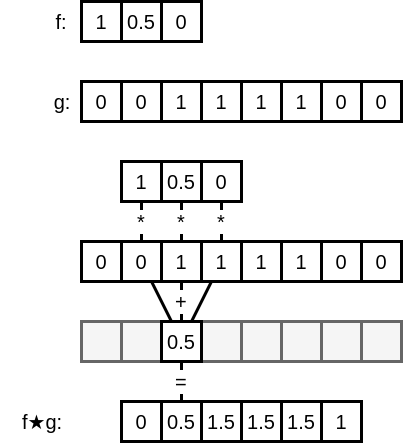
\includegraphics[height=0.7\textheight]{correlation.png}
    \end{figure}
\end{frame}

\begin{frame}{Discrete Autocorrelation}
    \begin{figure}
        \centering
        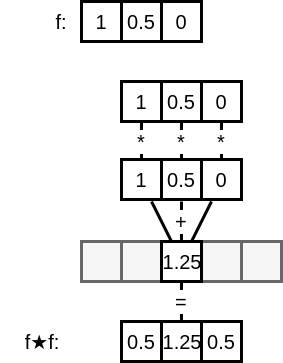
\includegraphics[height=0.7\textheight]{autocorrelation.png}
    \end{figure}
\end{frame}

\begin{frame}
\frametitle{Wavelets}
    \begin{itemize}
        \item Wavelet: A function that resembles a single oscillation of a wave
        \item Wavelets have both frequency and time domain info
        %\item Wavelet functions are sharper; can represent discontinuities efficiently
    \end{itemize}
    
    \begin{figure}
    \centering
    \begin{minipage}[b]{0.45\textwidth}
        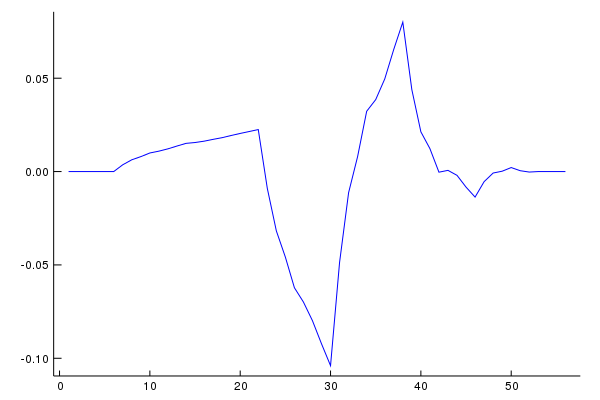
\includegraphics[width=\textwidth]{daub.png}
        \caption{Daubechies Wavelet}
    \end{minipage}
     \hfill
    \begin{minipage}[b]{0.45\textwidth}
        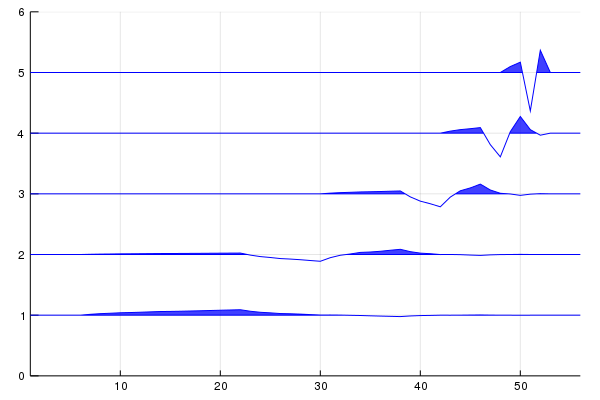
\includegraphics[width=\textwidth]{daub_wiggle.png}
        \caption{Daubechies Wavelets of various scales}
     \end{minipage}
    \end{figure}
\end{frame}

\begin{frame}{Wavelet Transforms}
    \begin{itemize}
        \item Represent a signal as a linear combination of wavelet basis functions
            \begin{align*}
                f(t) = \sum_{i=1}^n a_i \phi_i(t)
            \end{align*}
        where $a_i$ are expansion coefficients and $\phi(t)$ are the basis functions
        \item Wavelet transform deconstructs the signal using the same wavelet at different scales
        % \item We use the \emph{redundant} version of the wavelet transform called \emph{maximal overlap discrete wavelet transform} (MODWT), which gives us \emph{shift-invariant} representation of an input signal.
    \end{itemize}
\end{frame}

\begin{frame}
\frametitle{1D Autocorrelation Wavelet Transform}
    \begin{itemize}
        \item Redundant wavelet tranform
        \item Autocorrelation properties: shift-invariant \textbf{and} symmetric
    \end{itemize}
    Original Signal
    \begin{figure}
        \centering
        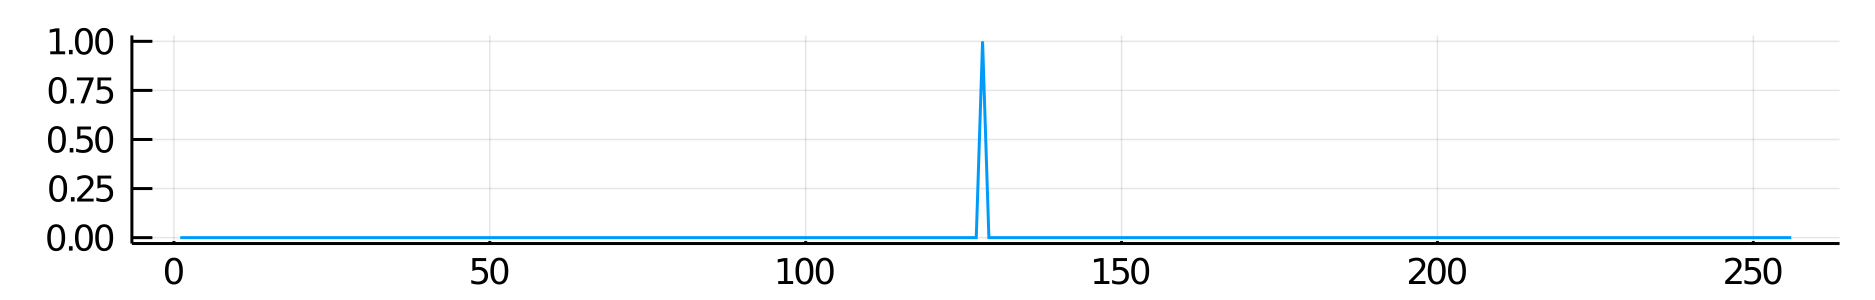
\includegraphics[width=0.57\textwidth,keepaspectratio]{spike_signal.png}
        % 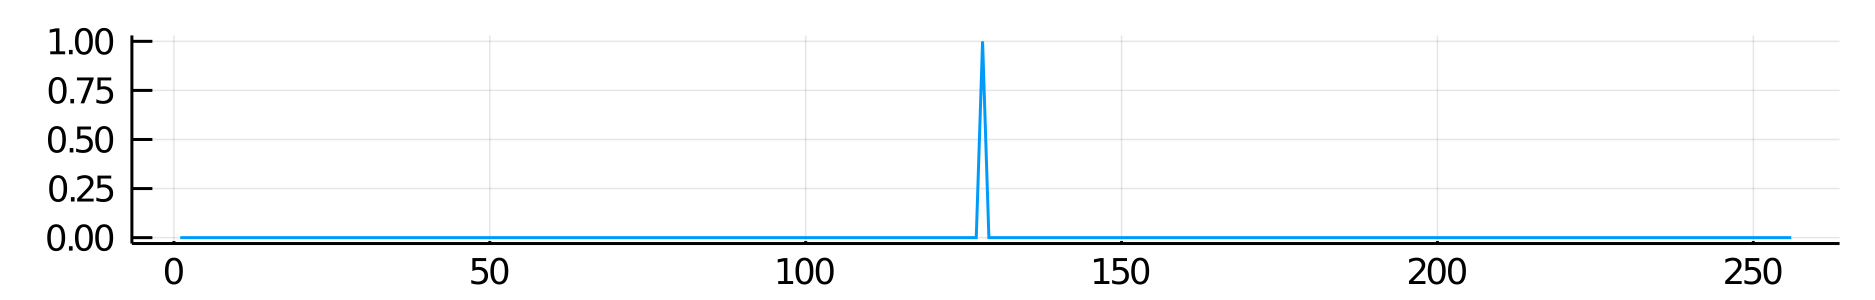
\includegraphics[height=0.2\textheight, width=0.6\textwidth]{spike_signal.png}
        % 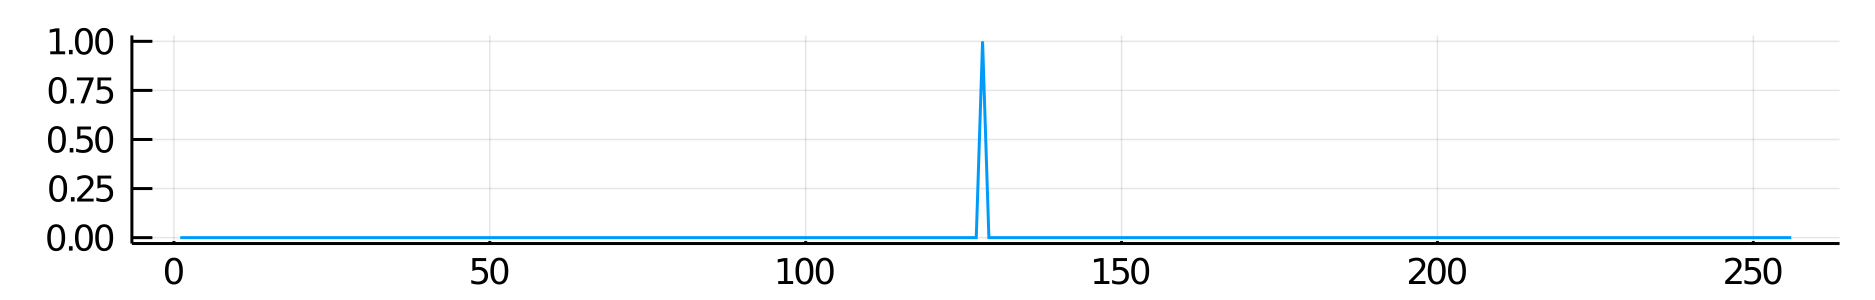
\includegraphics[scale=0.2]{spike_signal.png}
    \end{figure}
    
    Autocorrelation Functions of Wavelets
    \begin{figure}
        \centering
        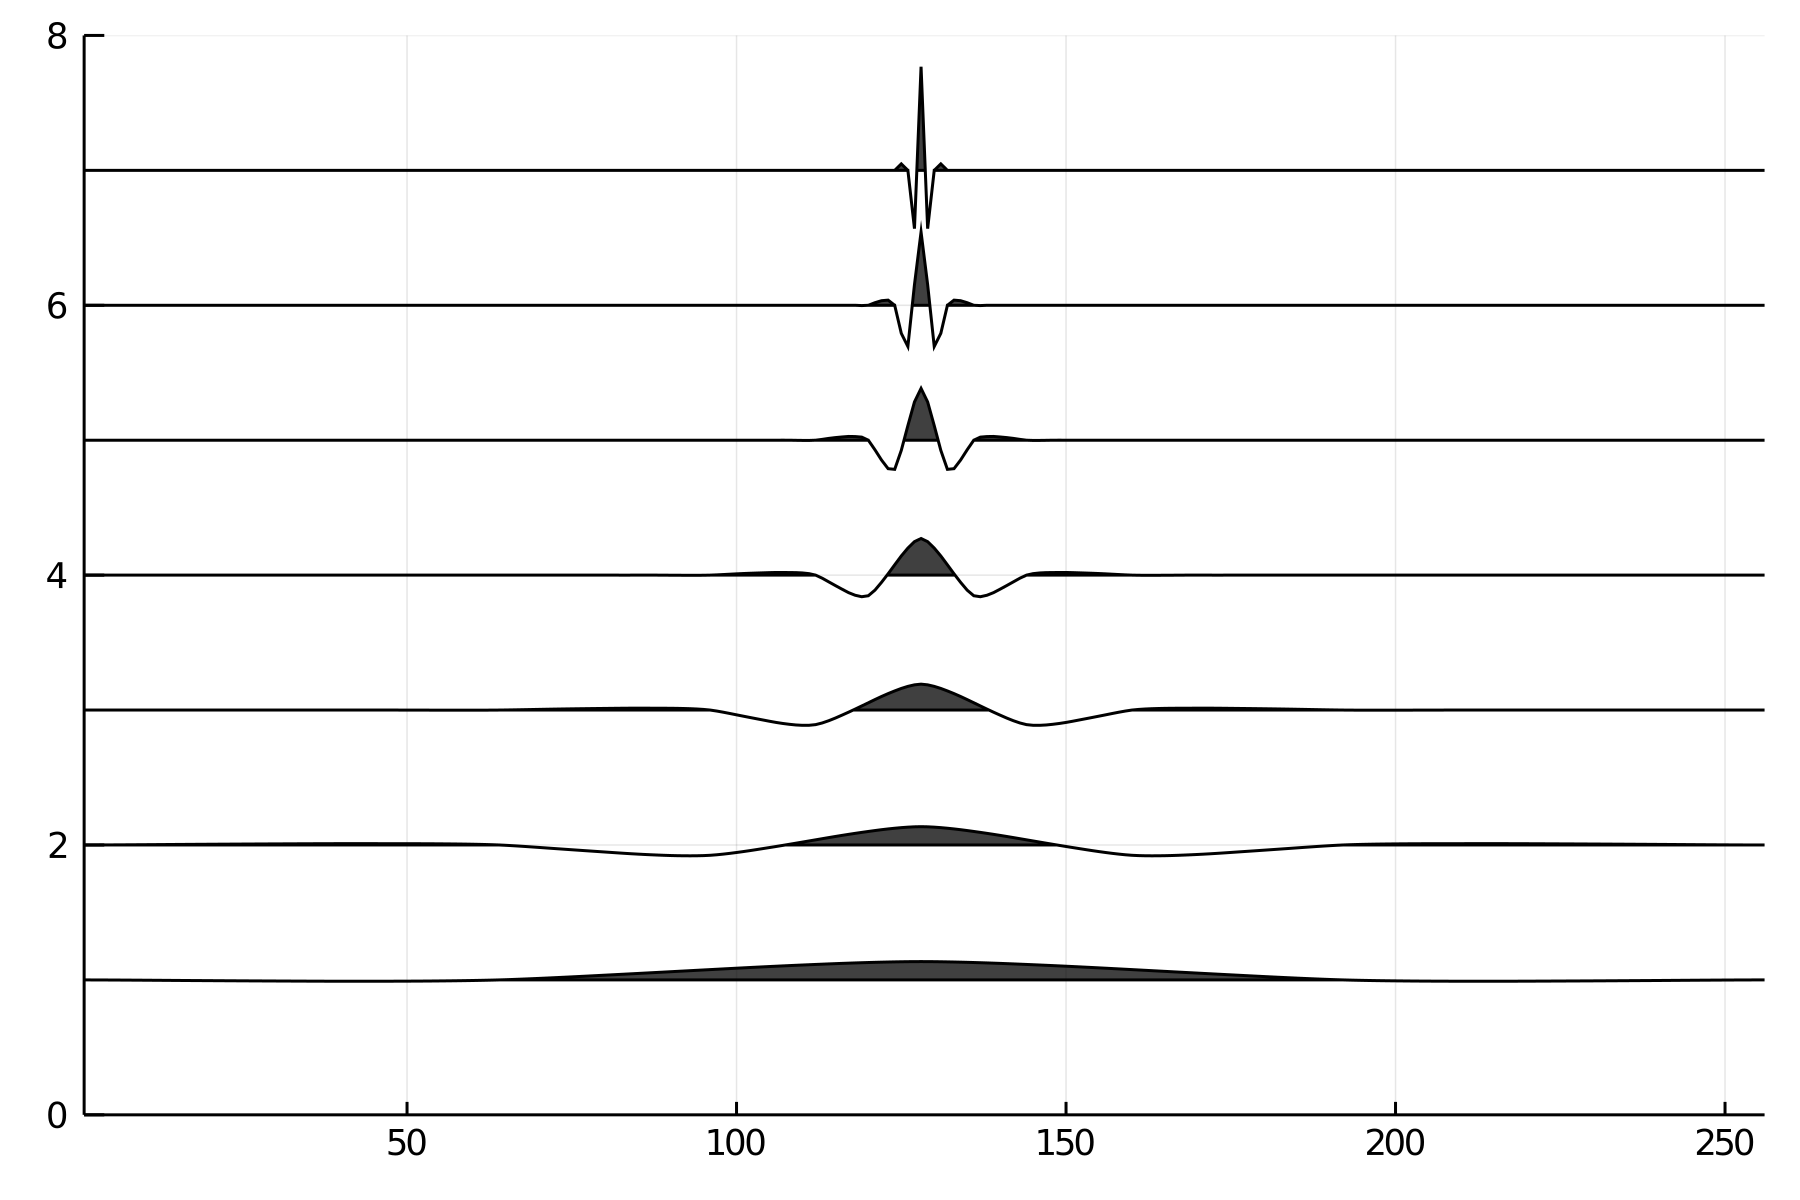
\includegraphics[ width=0.55\textwidth,height=0.45\textheight]{auto_decomposition.png}
        % 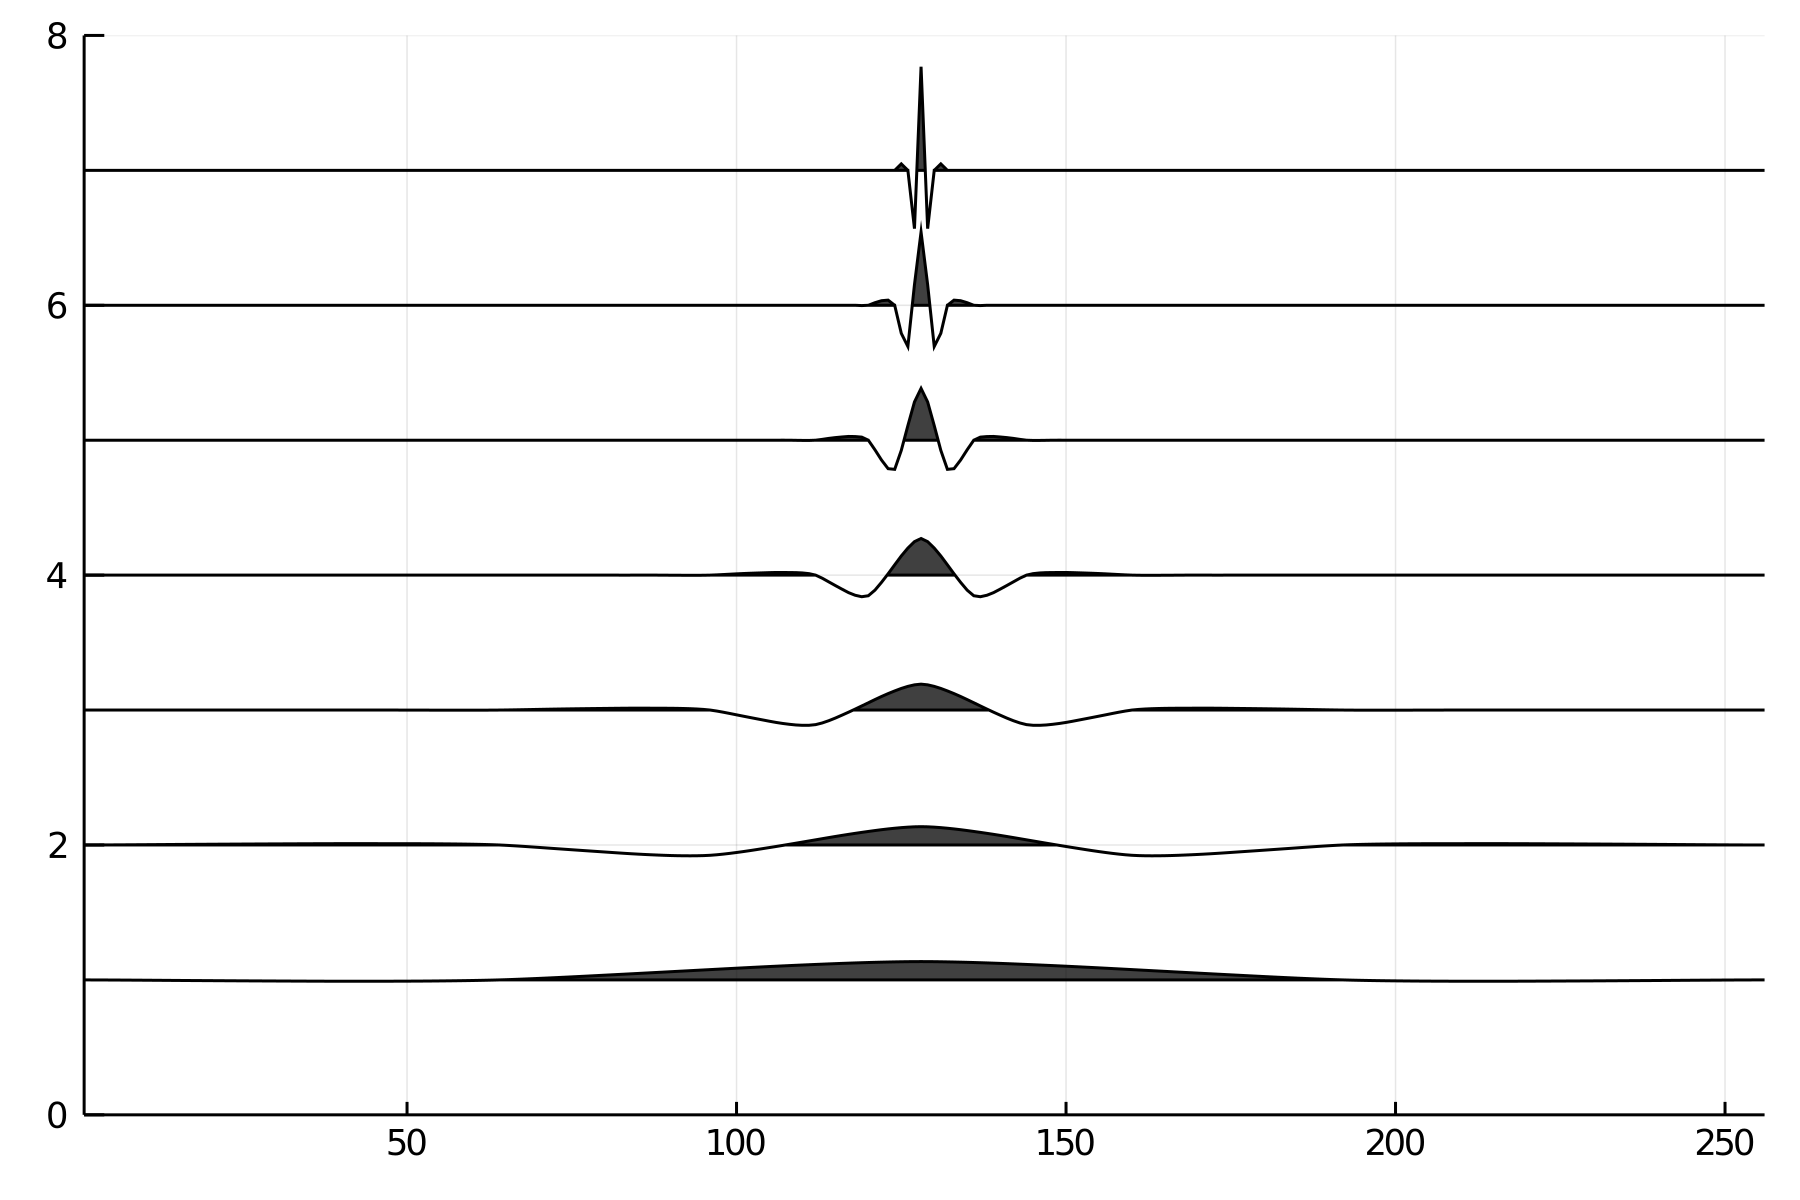
\includegraphics[height=0.5\textheight, width=0.6\textwidth]{auto_decomposition.png}
        % 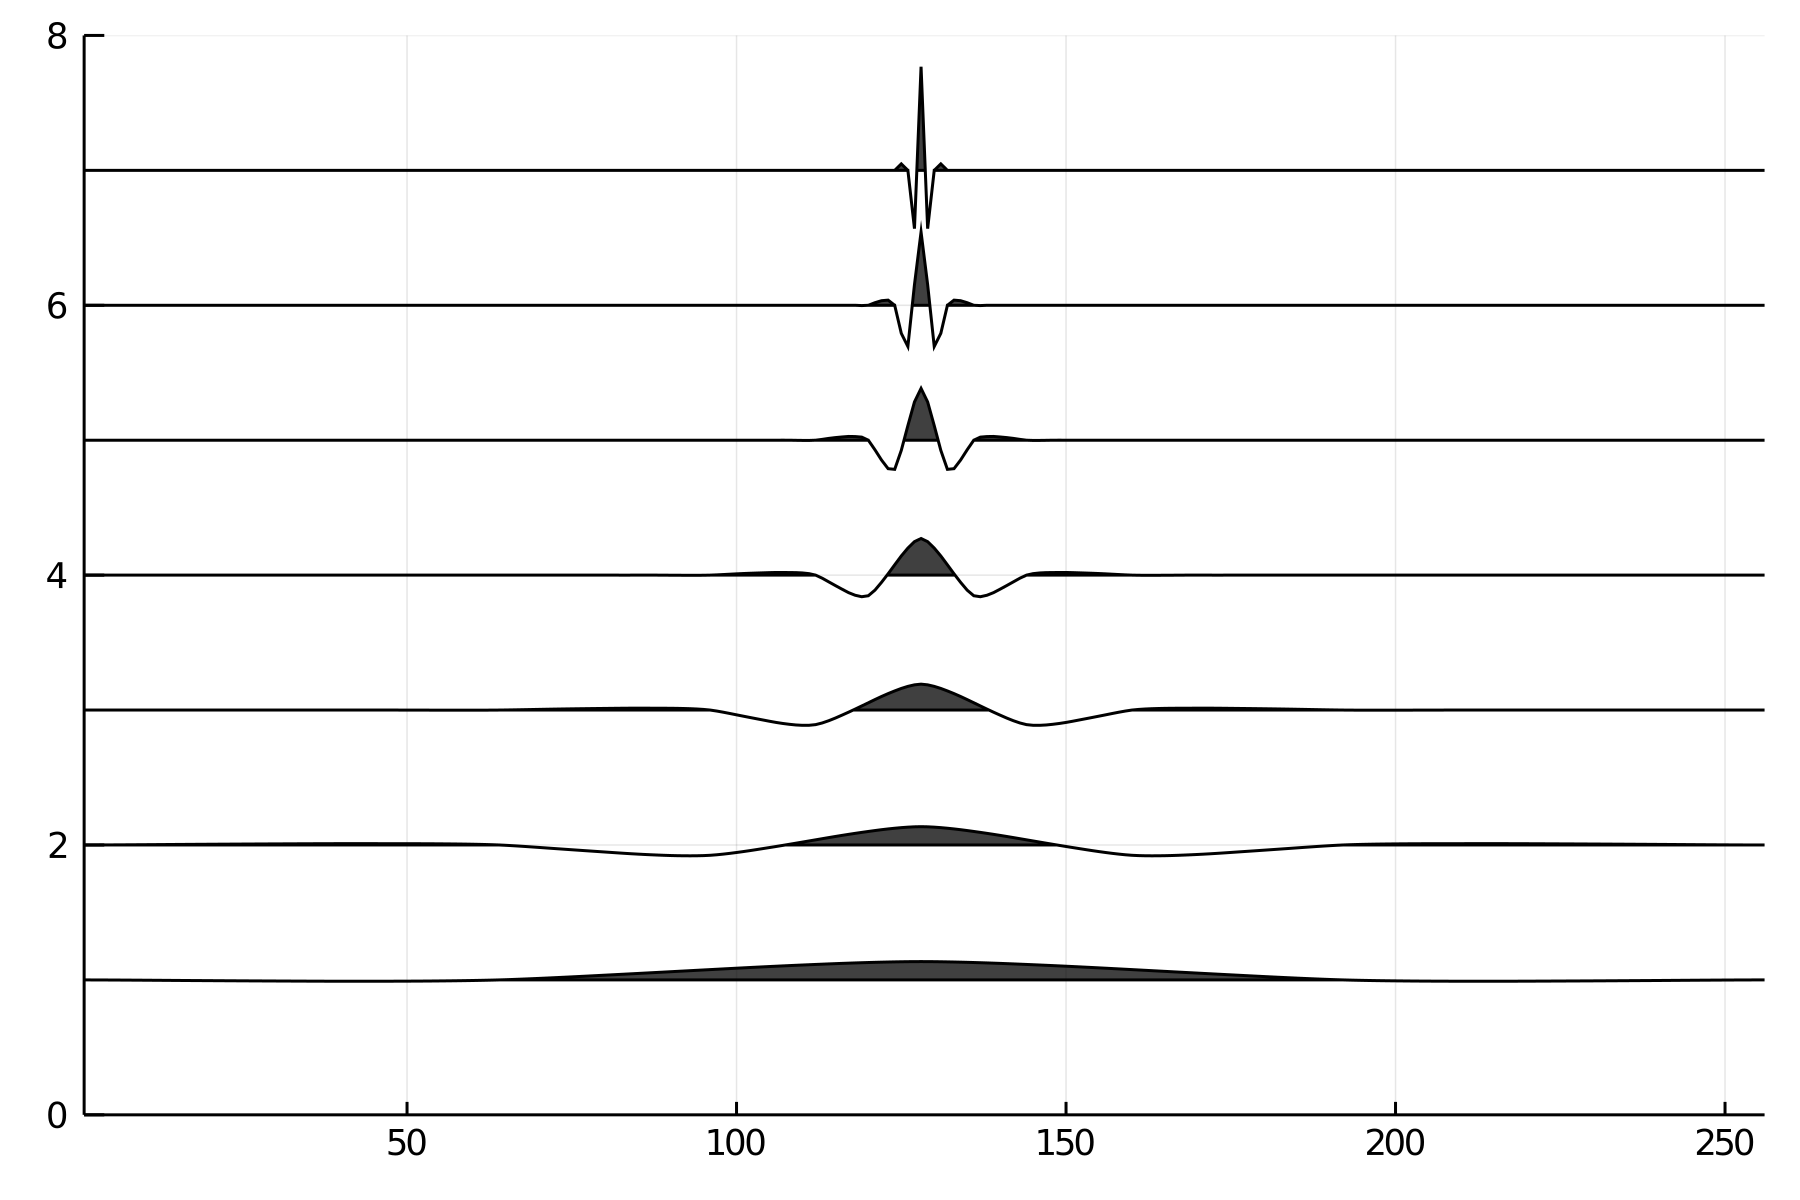
\includegraphics[scale=0.1]{auto_decomposition.png}
    \end{figure}
\end{frame}

\begin{frame}
\frametitle{2D Autocorrelation}
    \begin{figure}
        \centering
        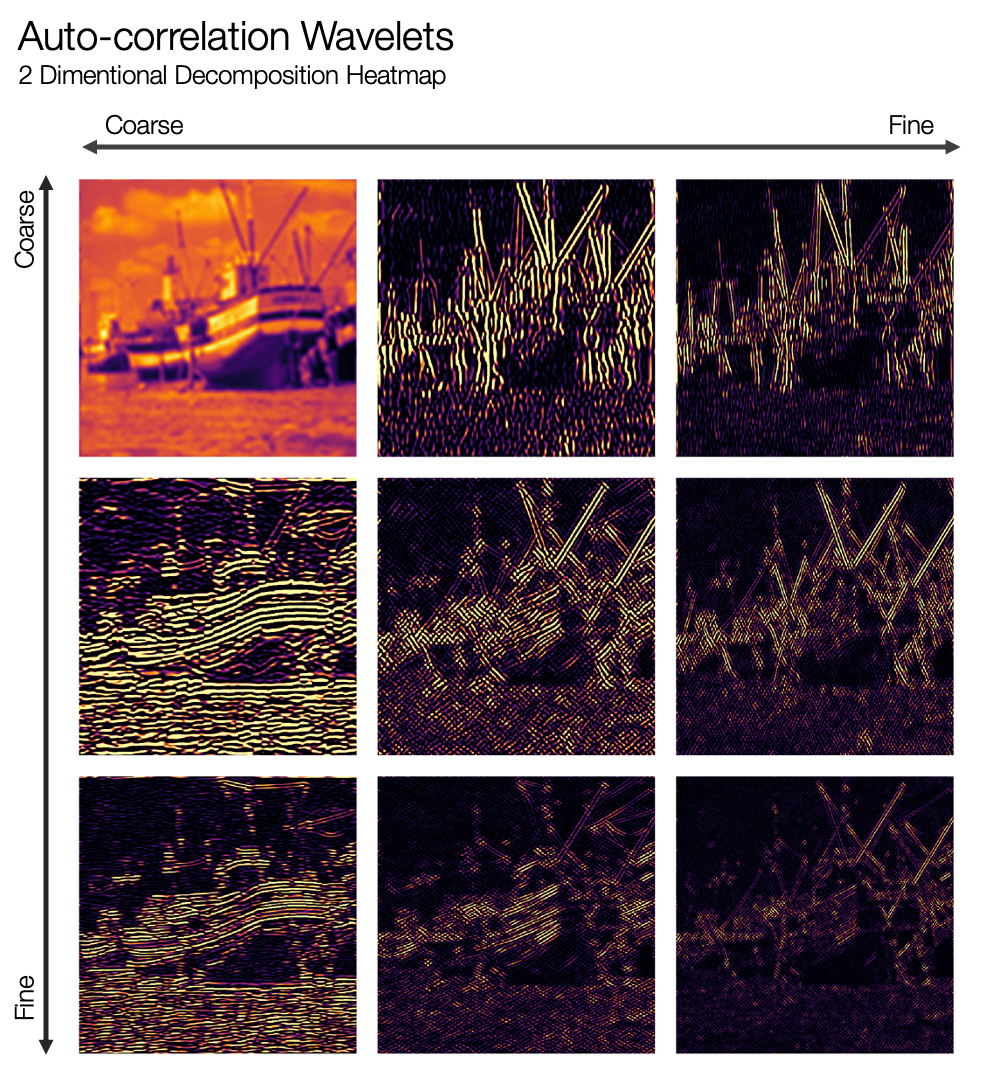
\includegraphics[height=7.5cm, keepaspectratio]{decomp_heatmap.png}
    \end{figure}
\end{frame}

\begin{frame}
\frametitle{Image De-noising}
    \begin{figure}
        \centering
        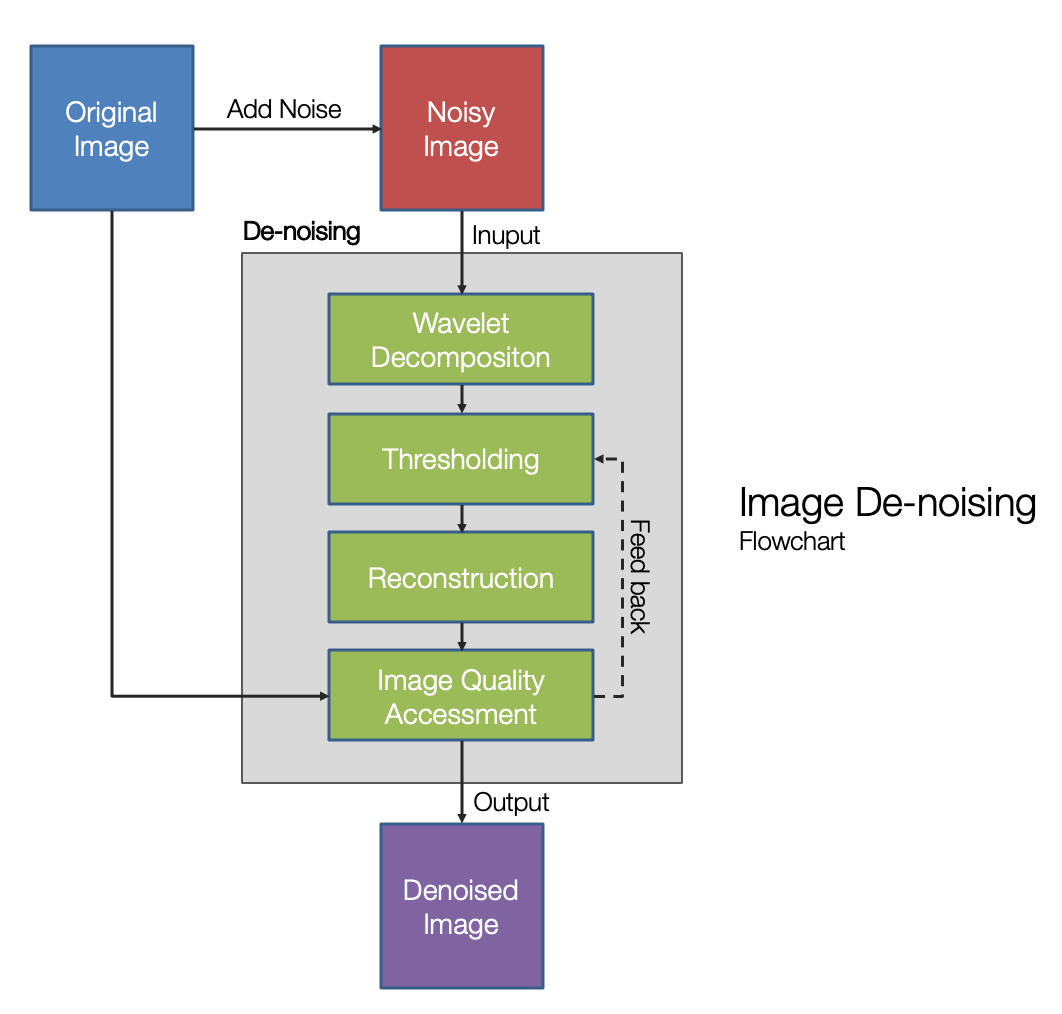
\includegraphics[height=0.8\textheight, keepaspectratio]{image_denoising.png}
    \end{figure}
\end{frame}

\begin{frame}
\frametitle{Image De-noising}
    \begin{figure}
        \centering
        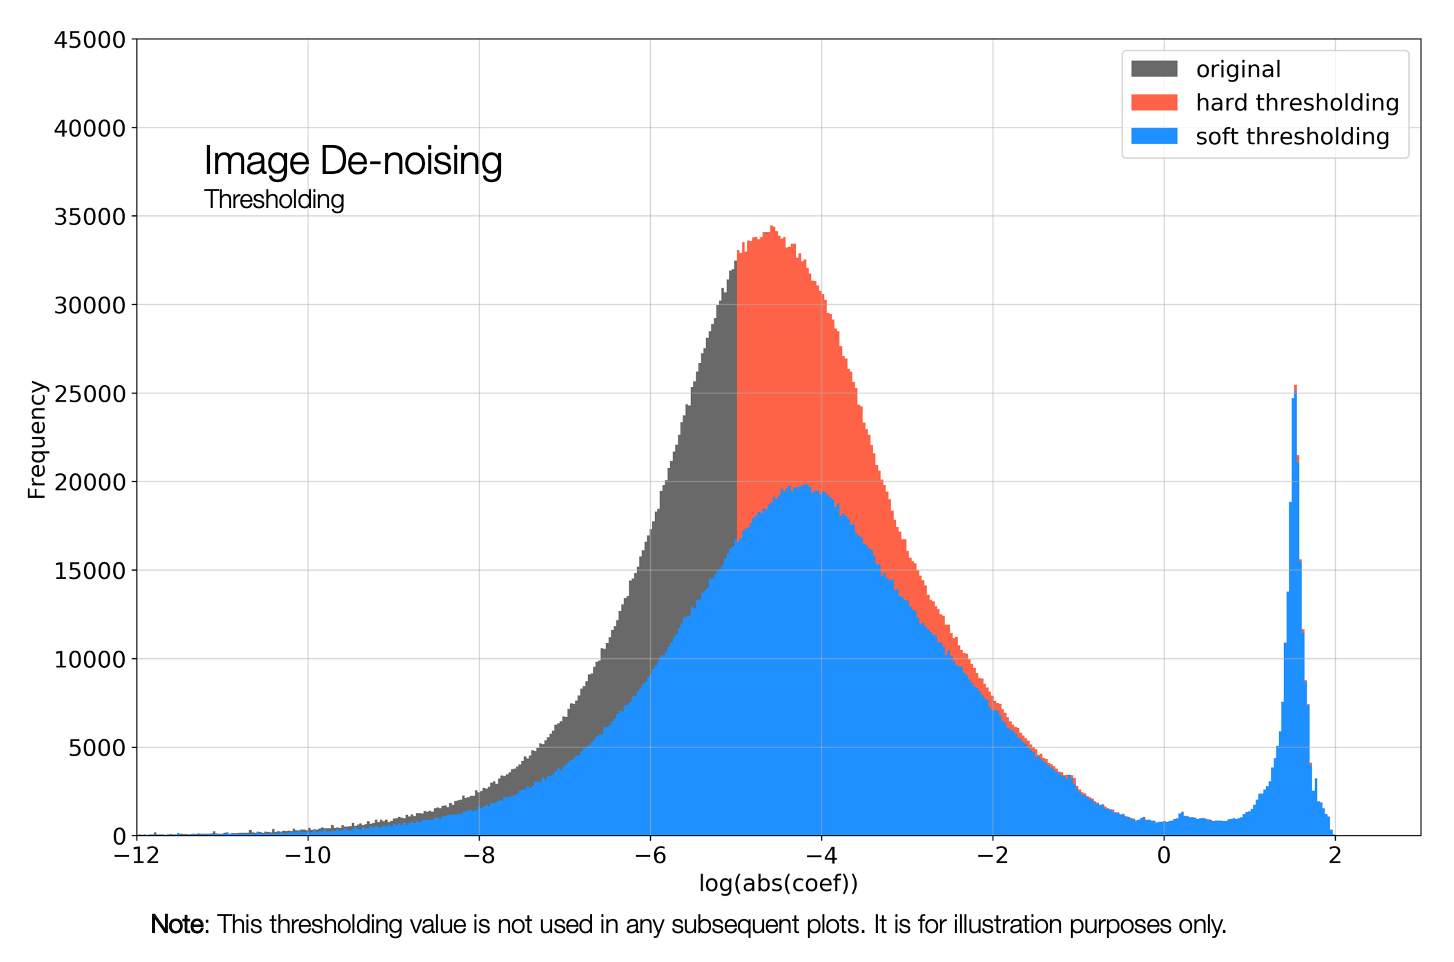
\includegraphics[height=0.8\textheight, keepaspectratio]{thresholding_plot.png}
    \end{figure}
\end{frame}

\begin{frame}
\frametitle{De-noising: Peak Signal to Noise Ratio (PSNR)}
Peak Signal to Noise Ratio (PSNR)
\begin{itemize}
    \item Ratio between maximum power of a signal and maximum power of corrupting noise
    \item Quantifies image quality degradation
\end{itemize}
\begin{equation}
    MSE = \frac{1}{mn}\sum_{i=0}^{m-1}\sum_{j=0}^{n-1}[I(i,j) - K(i,j)]^2
\end{equation}
\begin{equation}
    PSNR = 20\log_{10}\left(\frac{MAX_I}{\sqrt{MSE}}\right)
\end{equation}
\begin{itemize}
    \item $I, K, MAX_I$: original image, denoised image and the maximum possible pixel value of I
    \item The smaller the $MSE$, the larger the value
\end{itemize}
\end{frame}

\begin{frame}
\frametitle{De-noising: Peak Signal to Noise Ratio (PSNR)}
    \begin{figure}
        \centering
        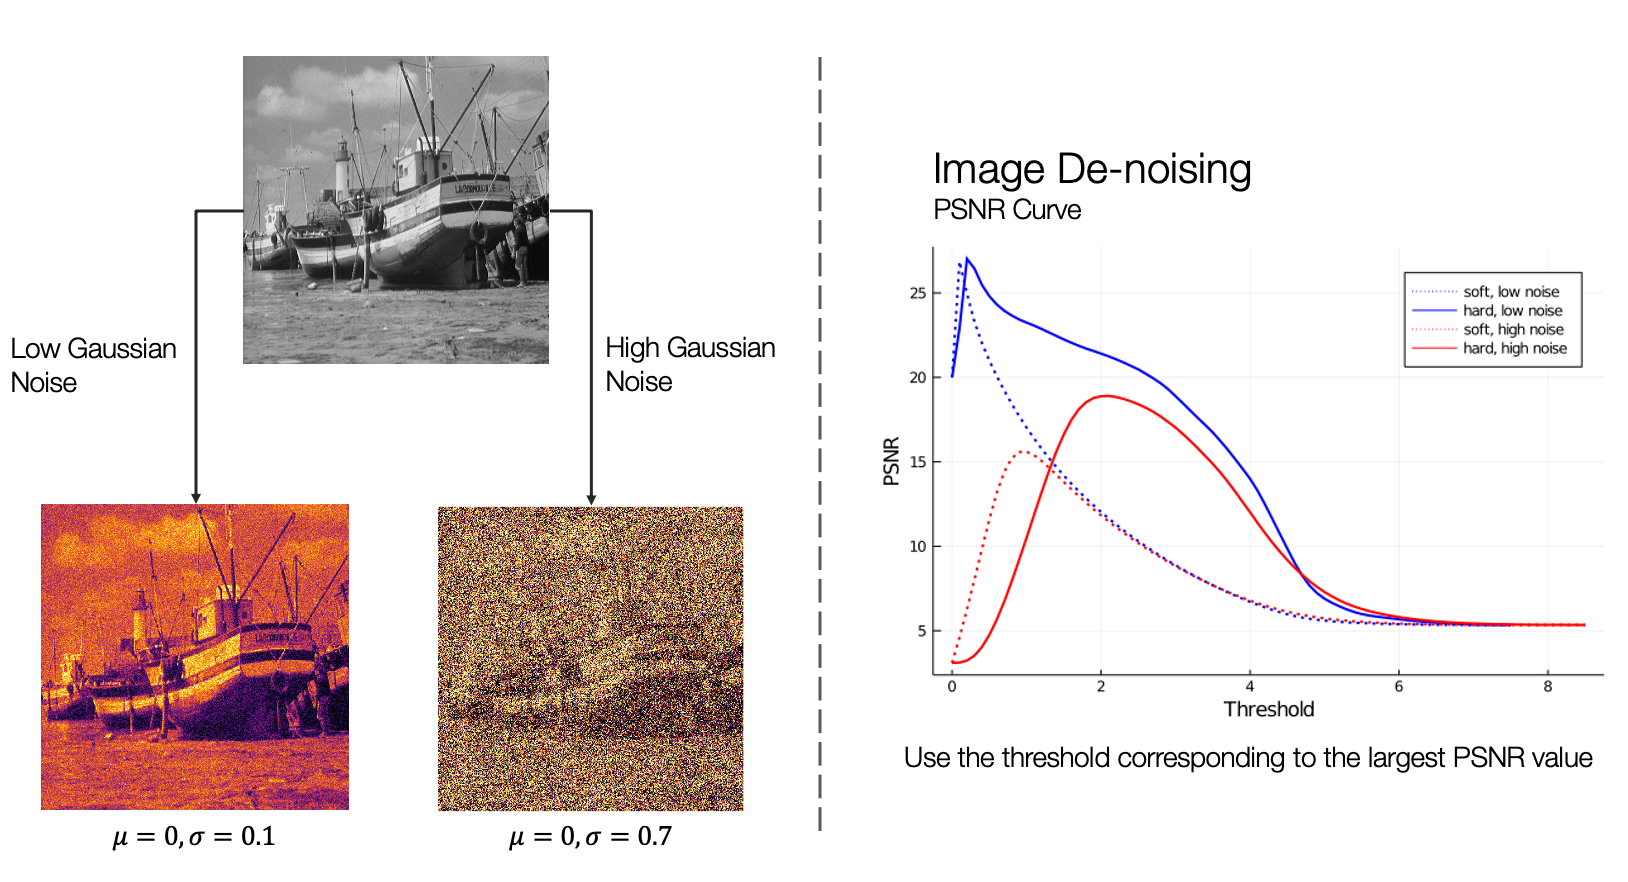
\includegraphics[height=0.85\textheight, keepaspectratio]{psnr_curve.png}
    \end{figure}
\end{frame}

\begin{frame}
\frametitle{De-noising: Peak Signal to Noise Ratio (PSNR)}
    \begin{figure}
        \centering
        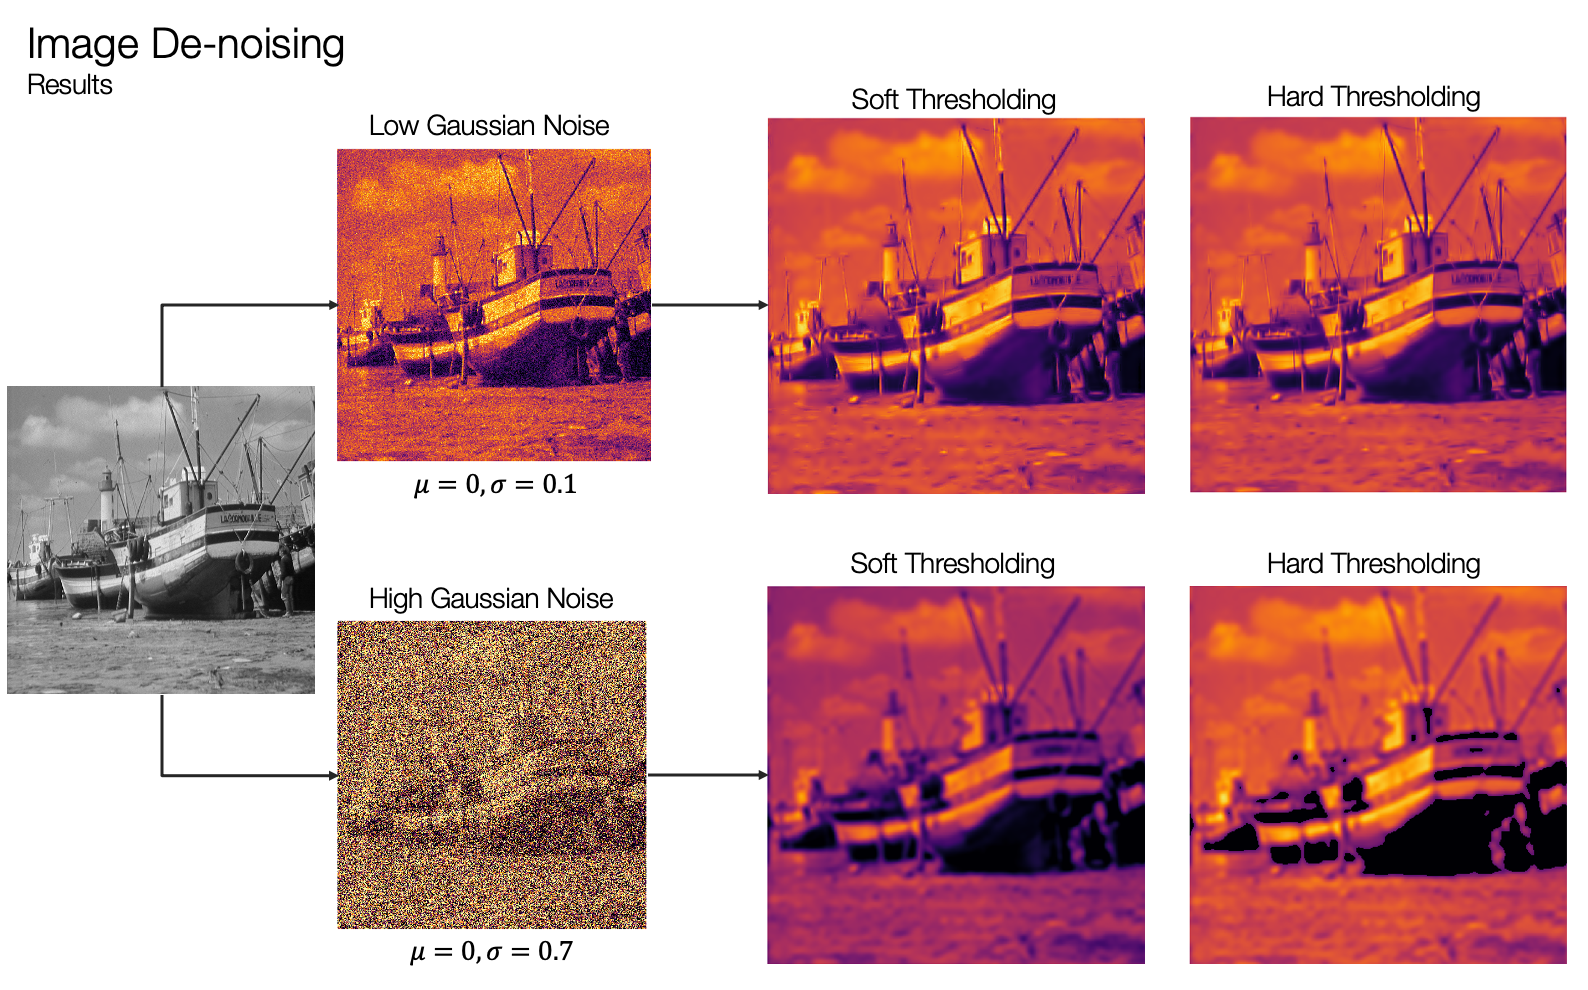
\includegraphics[height=0.85\textheight, keepaspectratio]{denoising_result.png}
    \end{figure}
\end{frame}

\begin{frame}
\frametitle{Data Analysis 1: Commodity Prices}
\begin{itemize}
    \item Commodity index: weighted average of the prices of a selected basket of goods relative to their prices in some base year
    %tracks the price and return on investment of a basket of commodities
    \item Source: International Monetary Fund
    \begin{itemize}
        \item Includes commodity indices such as Industrial Materials Index, Food Index, Energy Index, etc.
        \item Quarterly data which spans from 1992Q1 to 2020Q1 %113 time points
    \end{itemize}
    \item The indices are based in 2016
        \begin{itemize}
            \item Example  
        \end{itemize}
        \begin{align*}
            \text{Commodity Index for 2020} = \frac{\text{Price of Basket in 2020}}{\text{Price of Basket in 2016}} * 100
        \end{align*}
\end{itemize}
\end{frame}

\begin{frame}
\frametitle{Data Analysis 1: Commodity Prices}
\begin{figure}
    \centering
    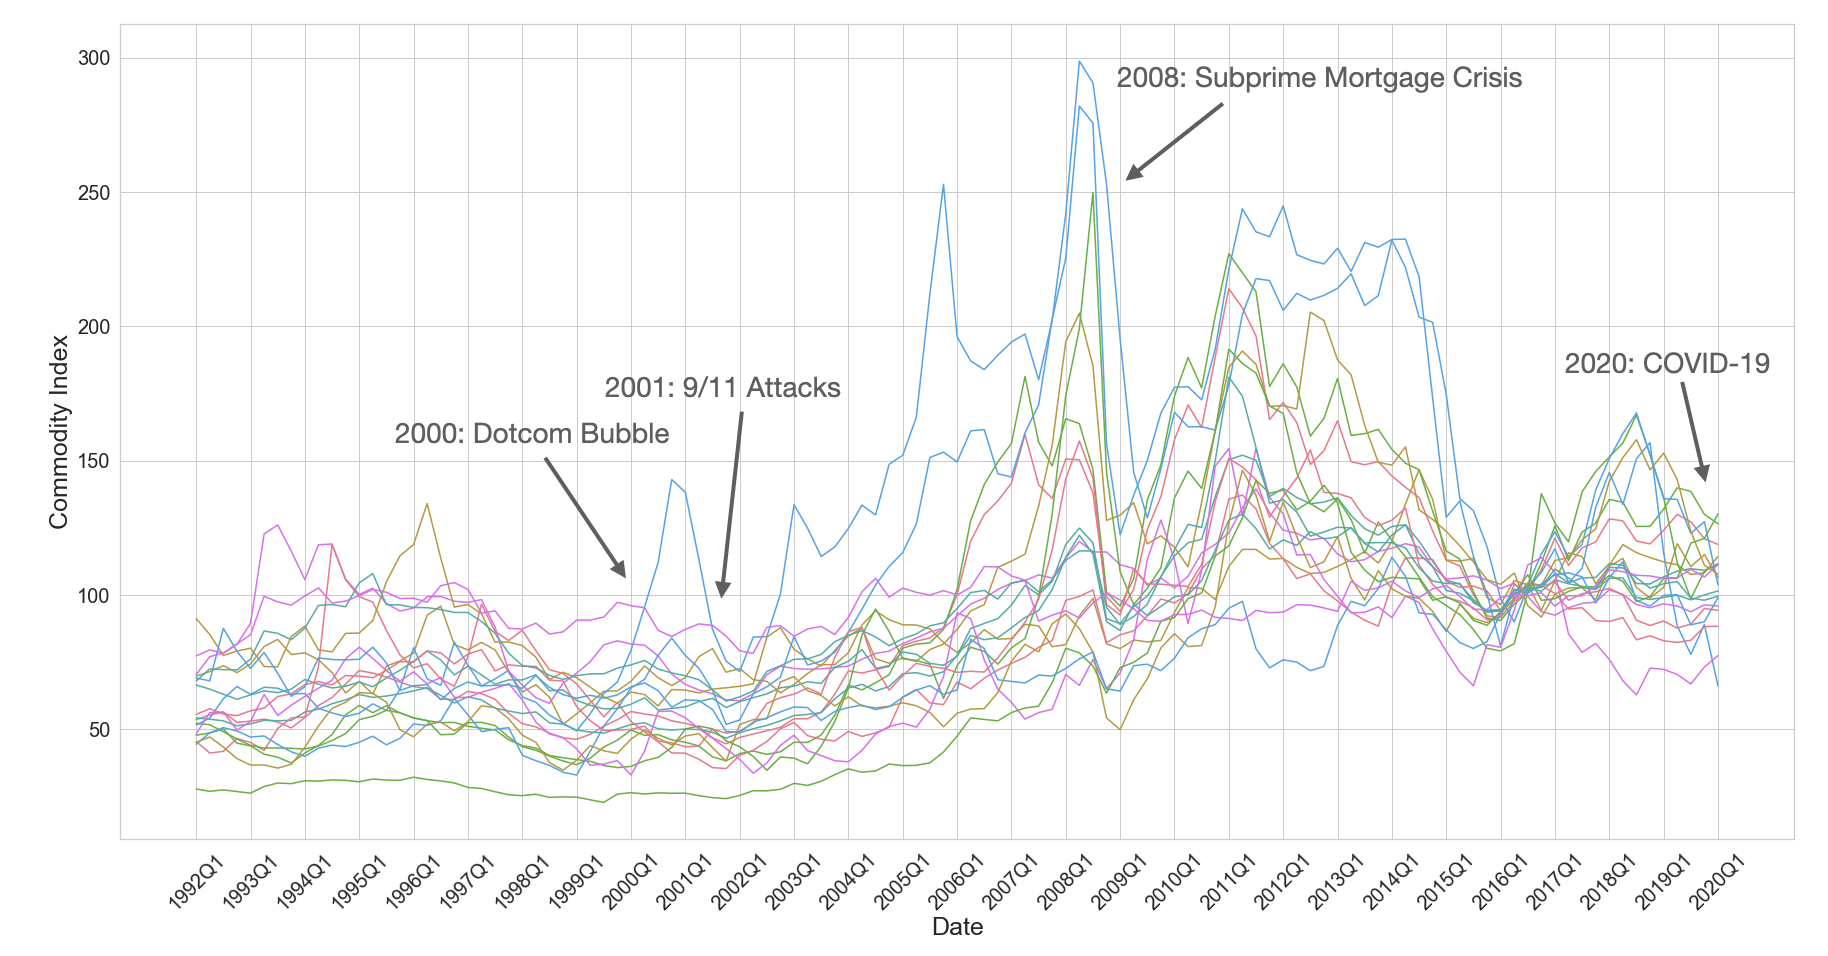
\includegraphics[scale=0.4]{comm.png}
\end{figure}
\end{frame}

\begin{frame}
\frametitle{Data Analysis 1: Commodity Prices}
\begin{itemize}
    \item Goal: denoise the data by thresholding the coefficients obtained from the autocorrelation wavelet transform
\end{itemize}
\begin{figure}
    \centering
    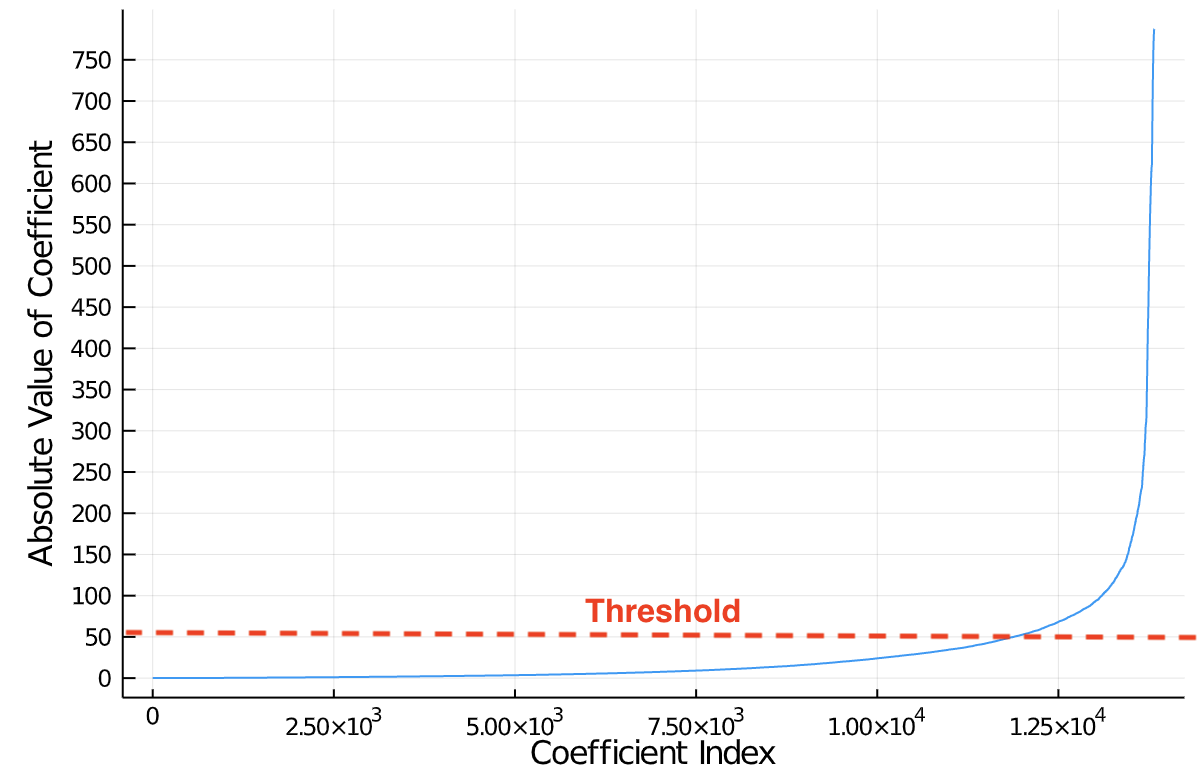
\includegraphics[scale=0.45]{comm_coef_thresh.png}
\end{figure}
\end{frame}

\begin{frame}
\frametitle{Data Analysis 1: Commodity Prices}
After thresholding:
\begin{figure}
    \centering
    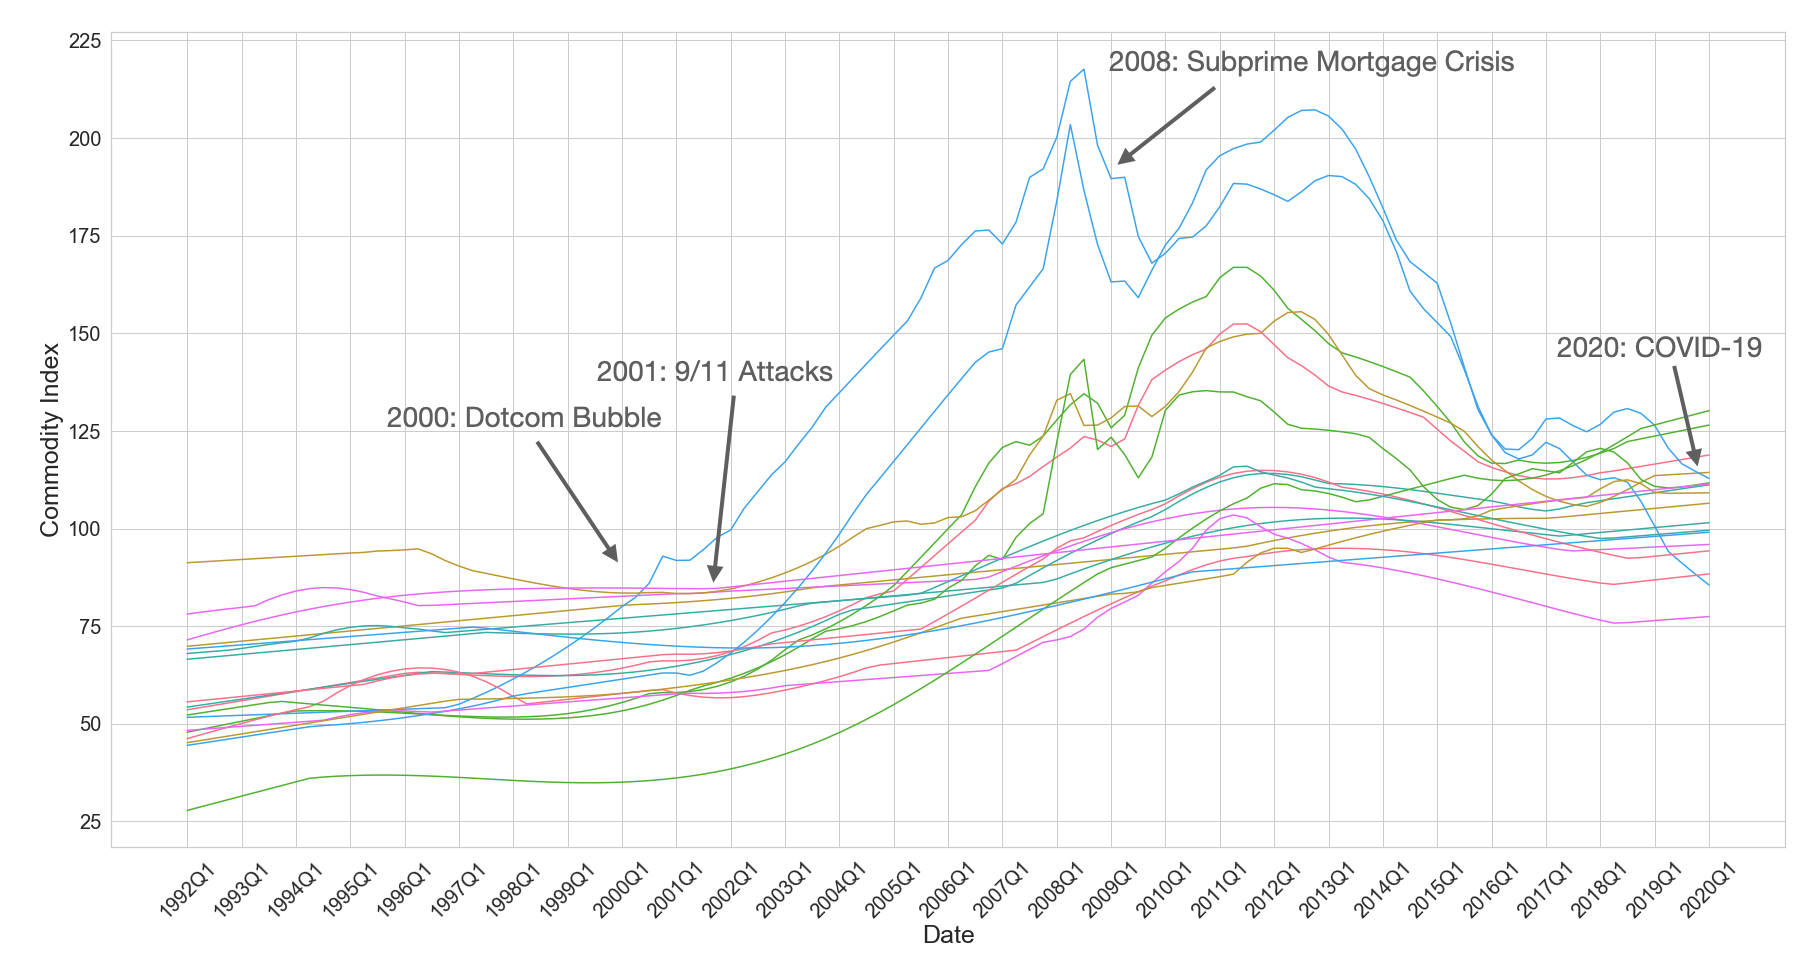
\includegraphics[scale=0.4]{comm_thresh.png}
\end{figure}
\end{frame}

% \begin{frame}
% \frametitle{Data Analysis 1: Commodity Prices}
% Before thresholding:
% \begin{figure}
%     \centering
%     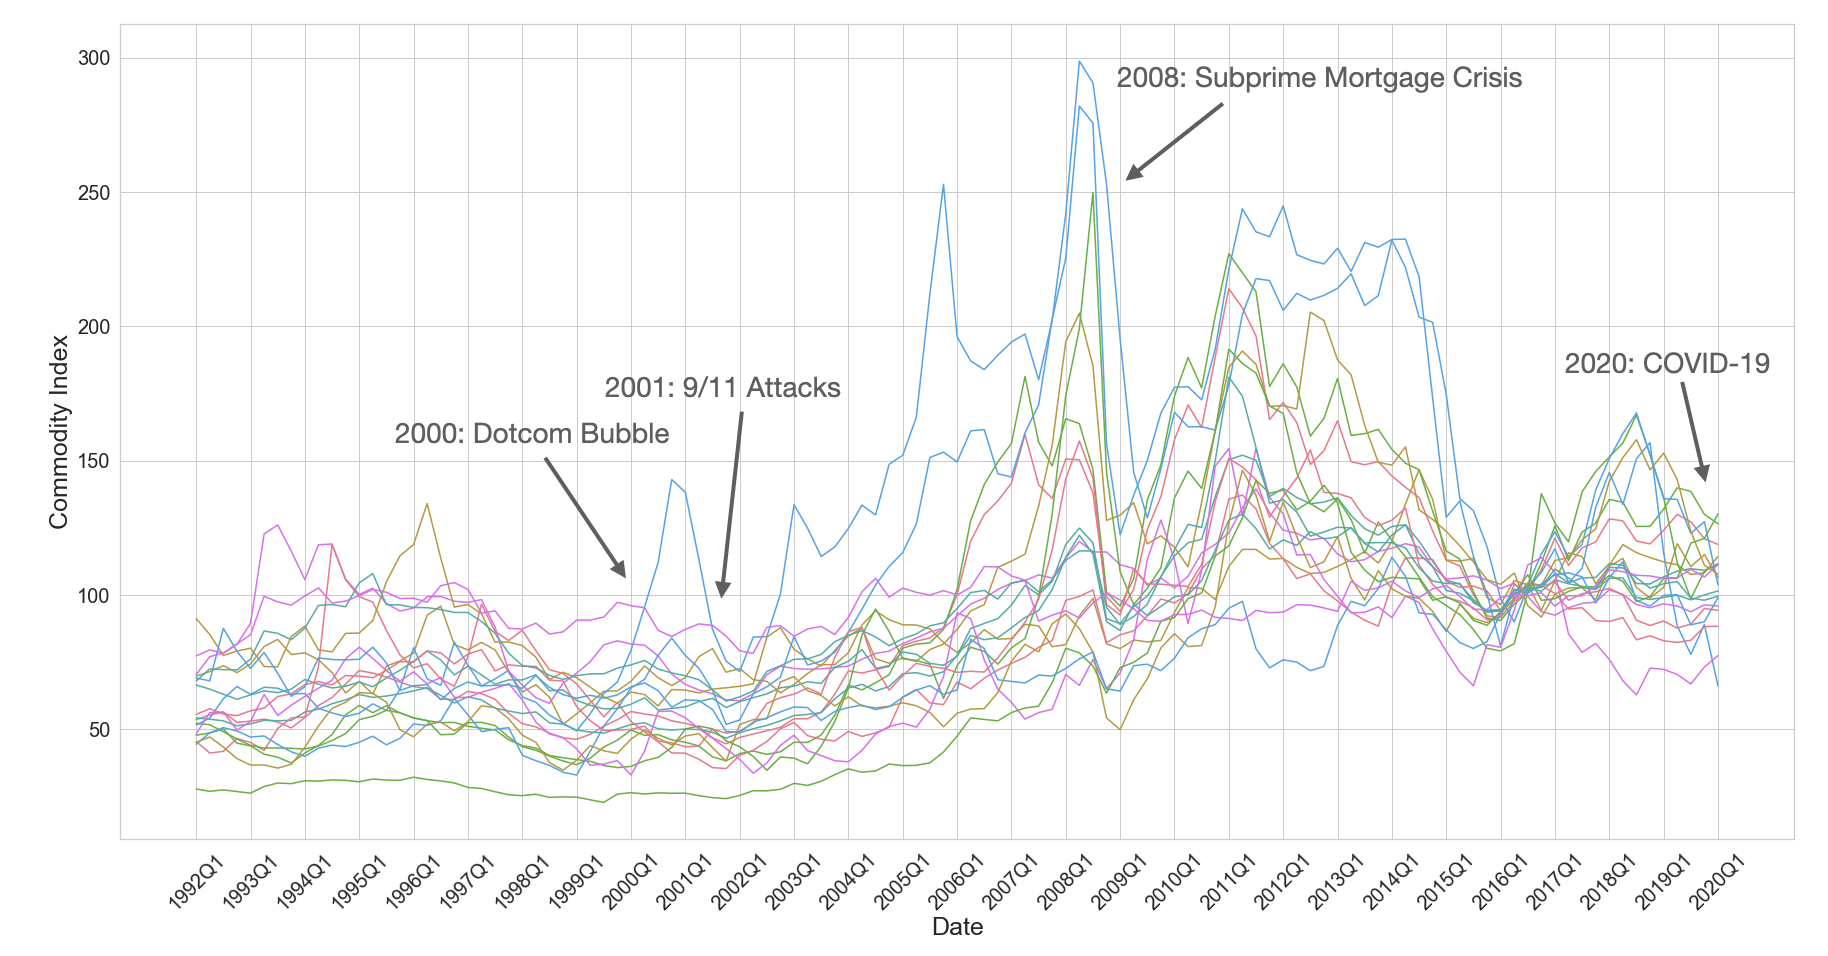
\includegraphics[scale=0.4]{comm.png}
% \end{figure}
% \end{frame}

\begin{frame}
\frametitle{Data Analysis 2: Floating Population}
Floating Population Data
\begin{itemize}
    \item Source: Tokyo Public Transportation Open Data Challenge
    \begin{itemize}
        \item Agoop: Subsidiary of SoftBank(Largest network provider in Japan)
    \end{itemize}
    \item Smart Phone Log Data (2018/10 to 2019/10)
    \begin{itemize}
        \item Date
        \item Location
        \item Gender
        \item Various Settings e.g. Currency, Language, Country
    \end{itemize}
    \item Goal: Use 2D auto-correlation wavelet decomposition to find trends in the flow of people.
\end{itemize}
\end{frame}

\begin{frame}
\frametitle{Data Analysis 2: Floating Population}
    \begin{figure}
        \centering
        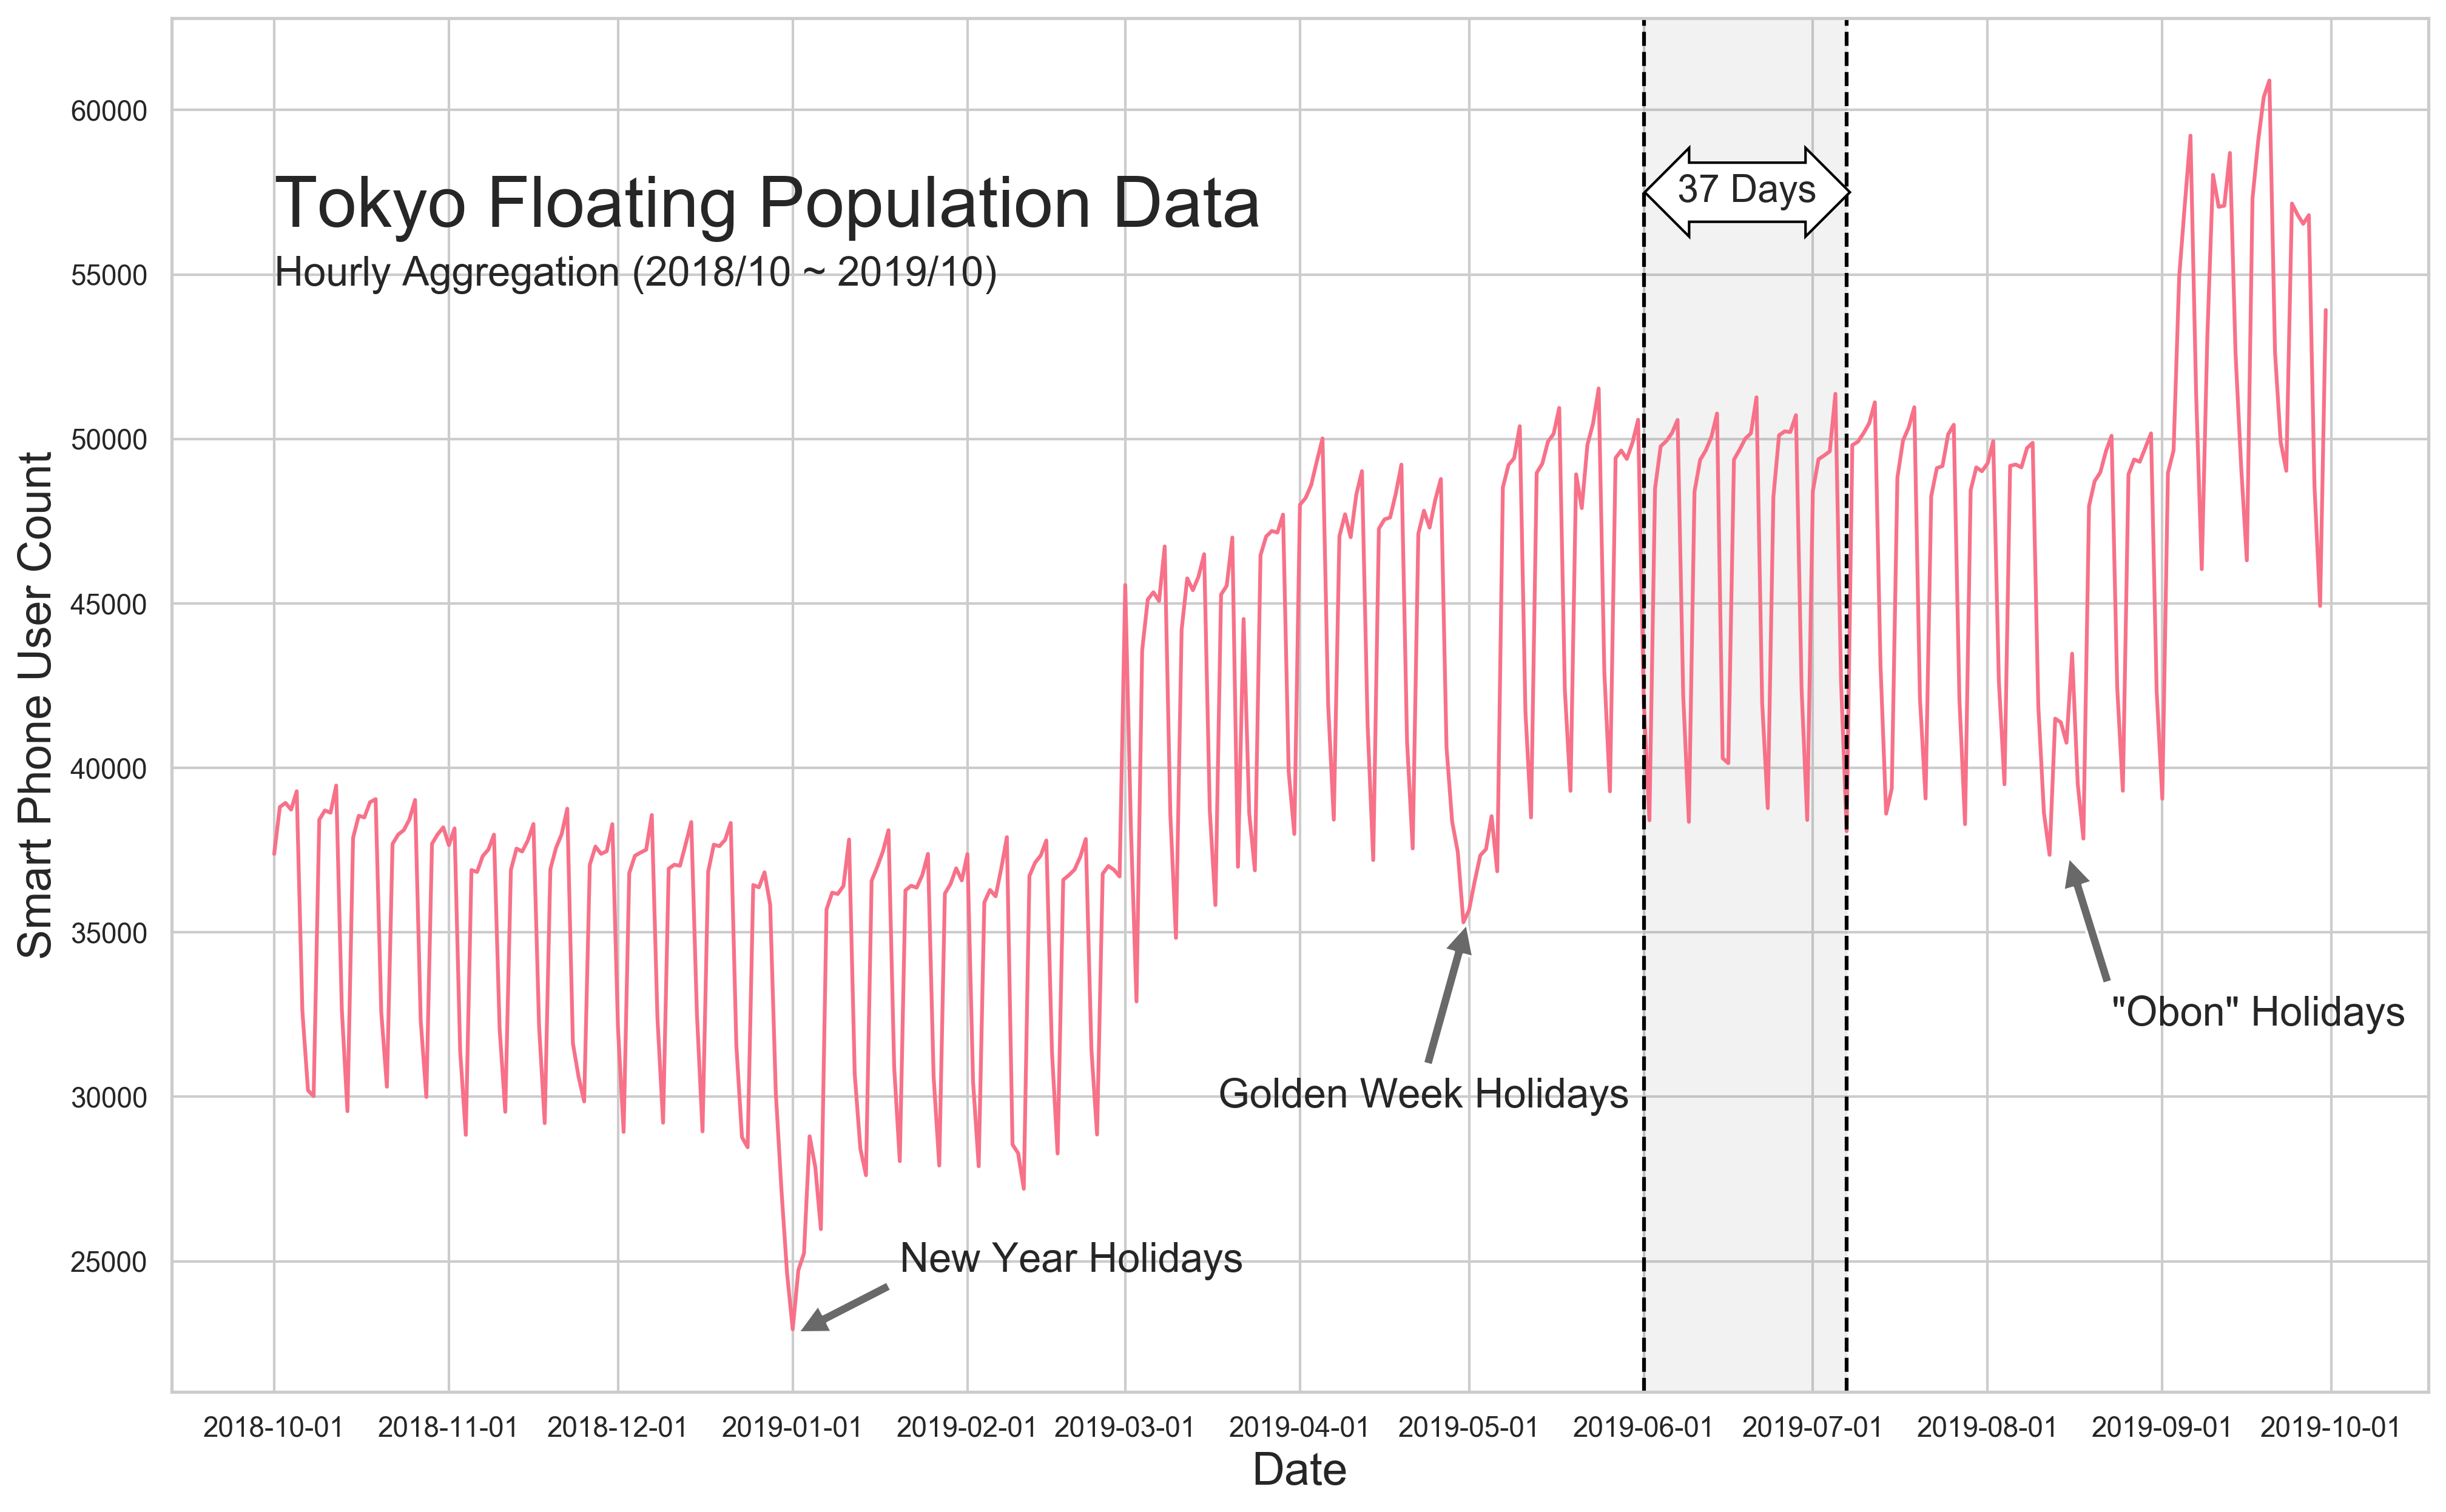
\includegraphics[height=0.85\textheight,width=0.85\textwidth]{images/Tokyo Float Pop Data.png}
    \end{figure}
\end{frame}

\begin{frame}{Data Analysis 2: Floating Population}
    \begin{figure}
        \centering
        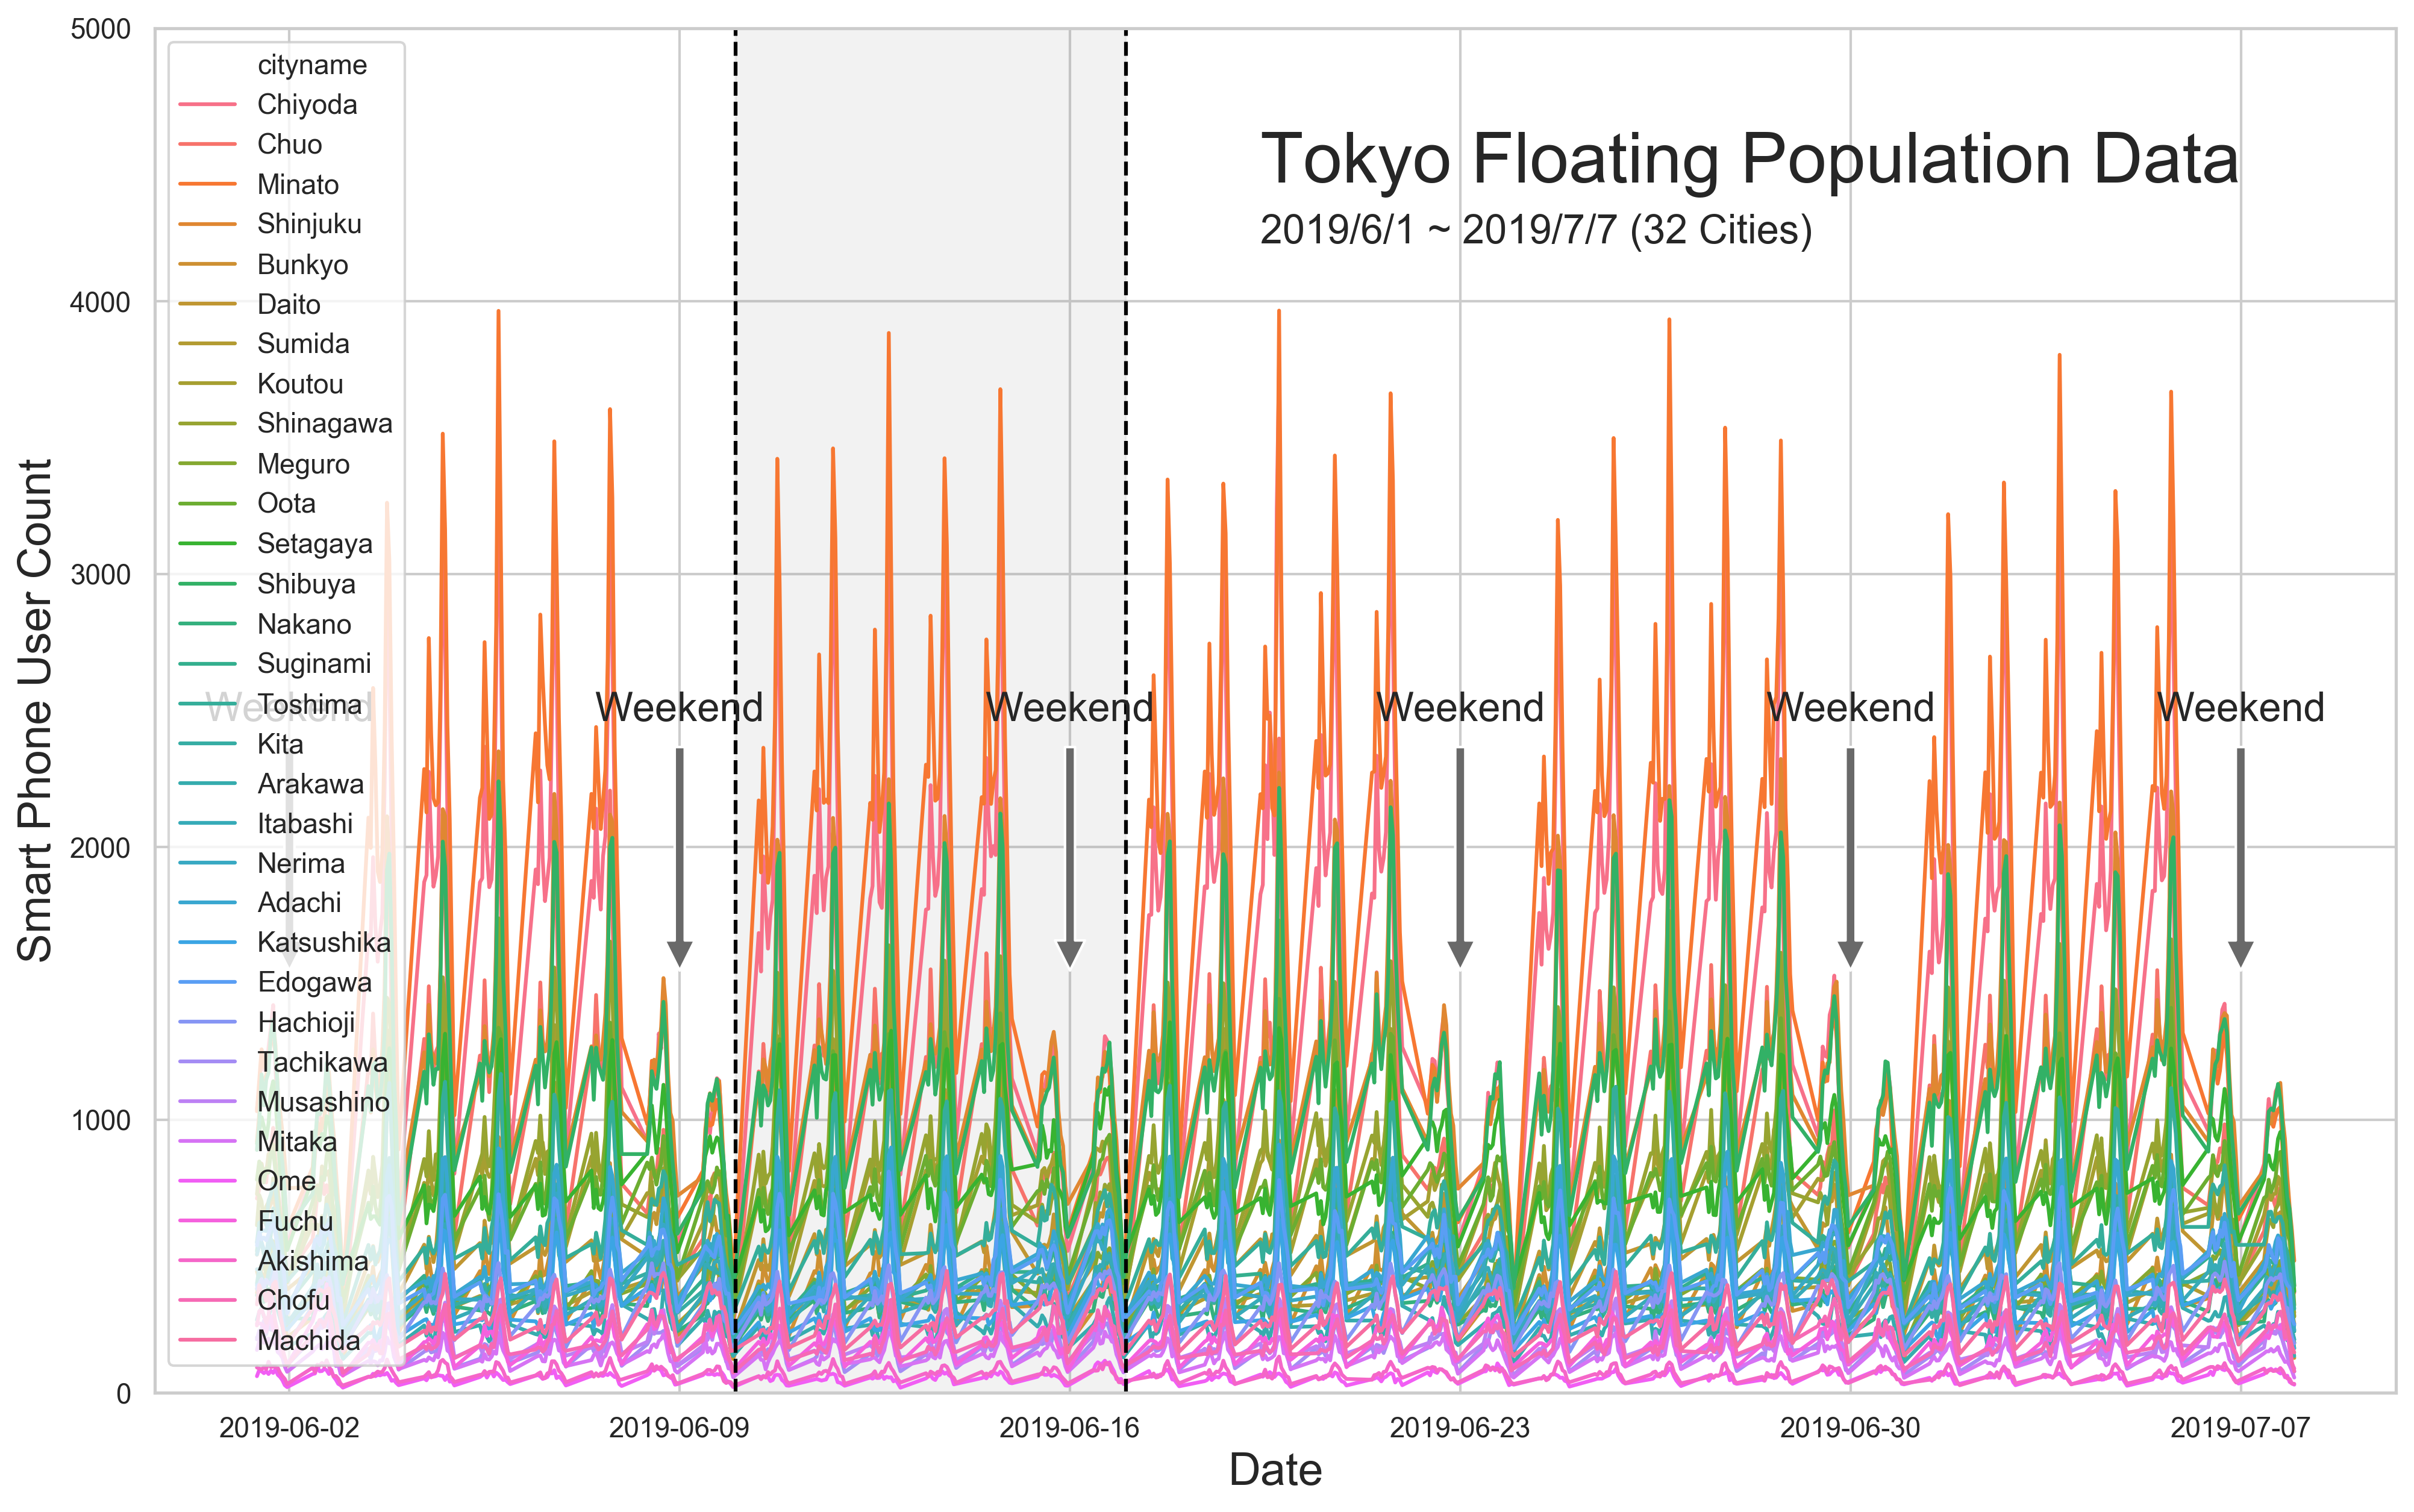
\includegraphics[height=0.85\textheight,width=0.85\textwidth]{images/Tokyo Float Pop 32.png}
    \end{figure}
\end{frame}

\begin{frame}{Data Analysis 2: Floating Population}
    \begin{figure}
        \centering
        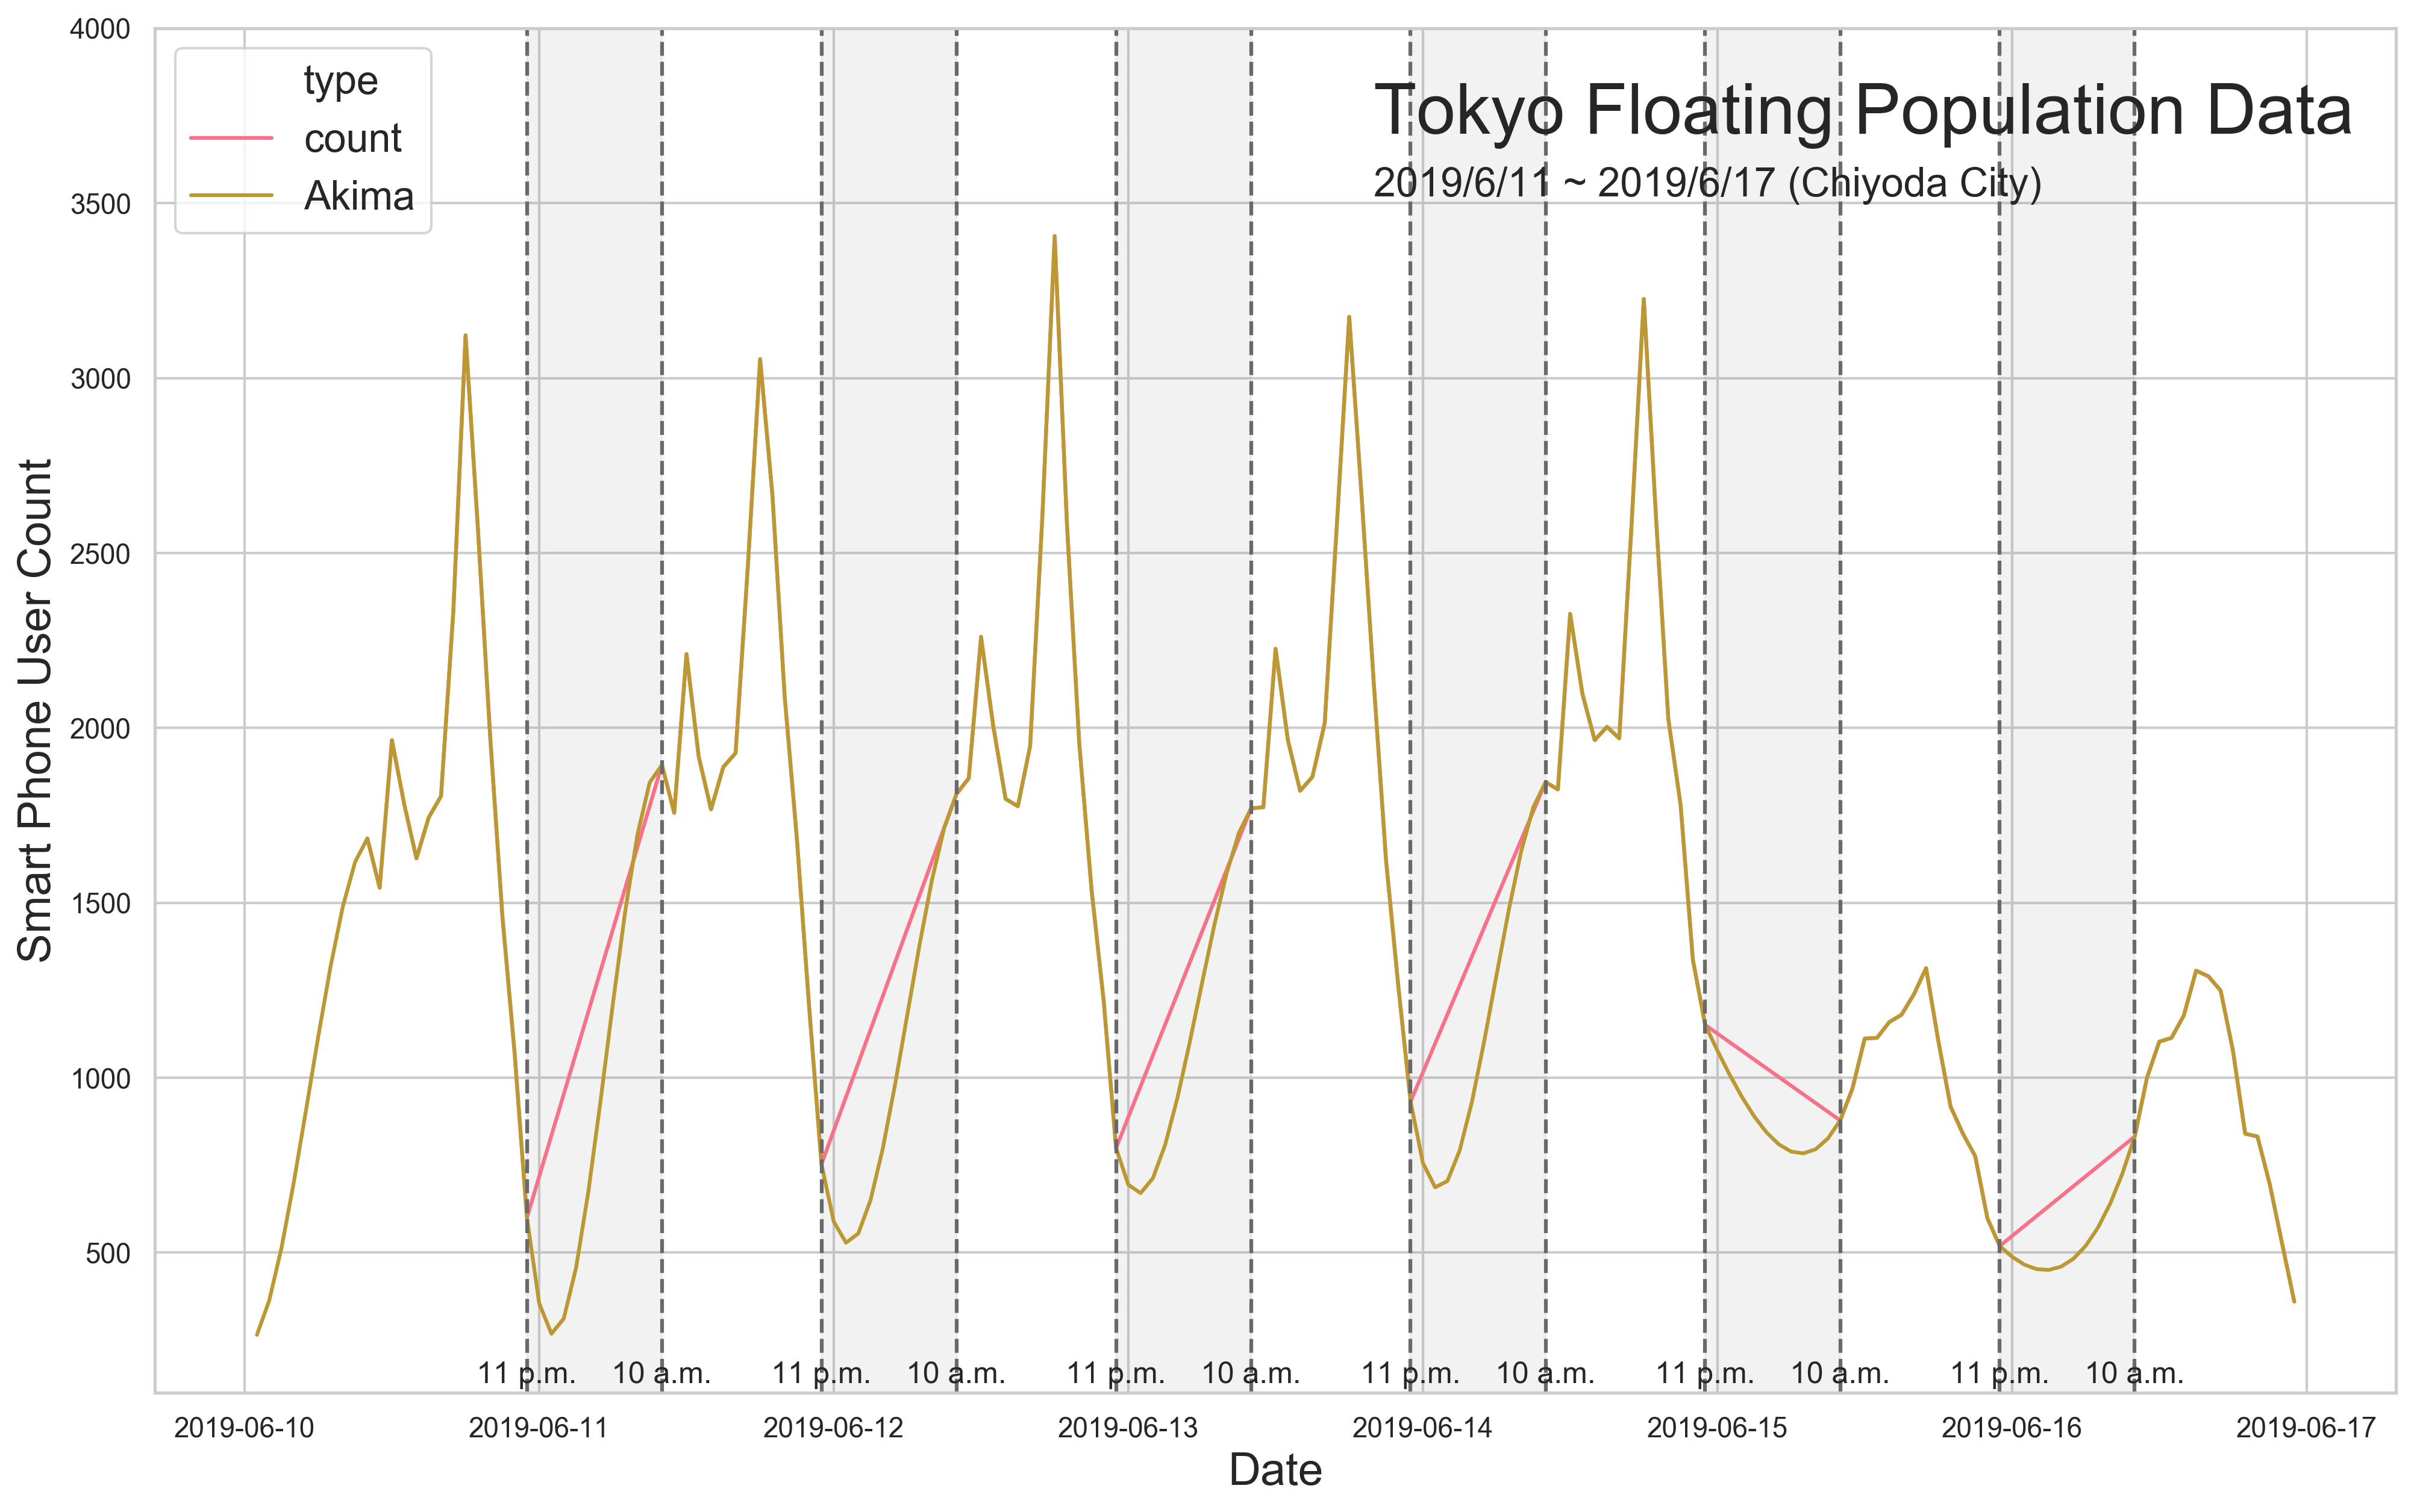
\includegraphics[height=0.85\textheight,width=0.85\textwidth]{images/Interpolate Akima.png}
    \end{figure}
\end{frame}

\begin{frame}{Data Analysis 2: Floating Population}
    \begin{figure}
        \centering
        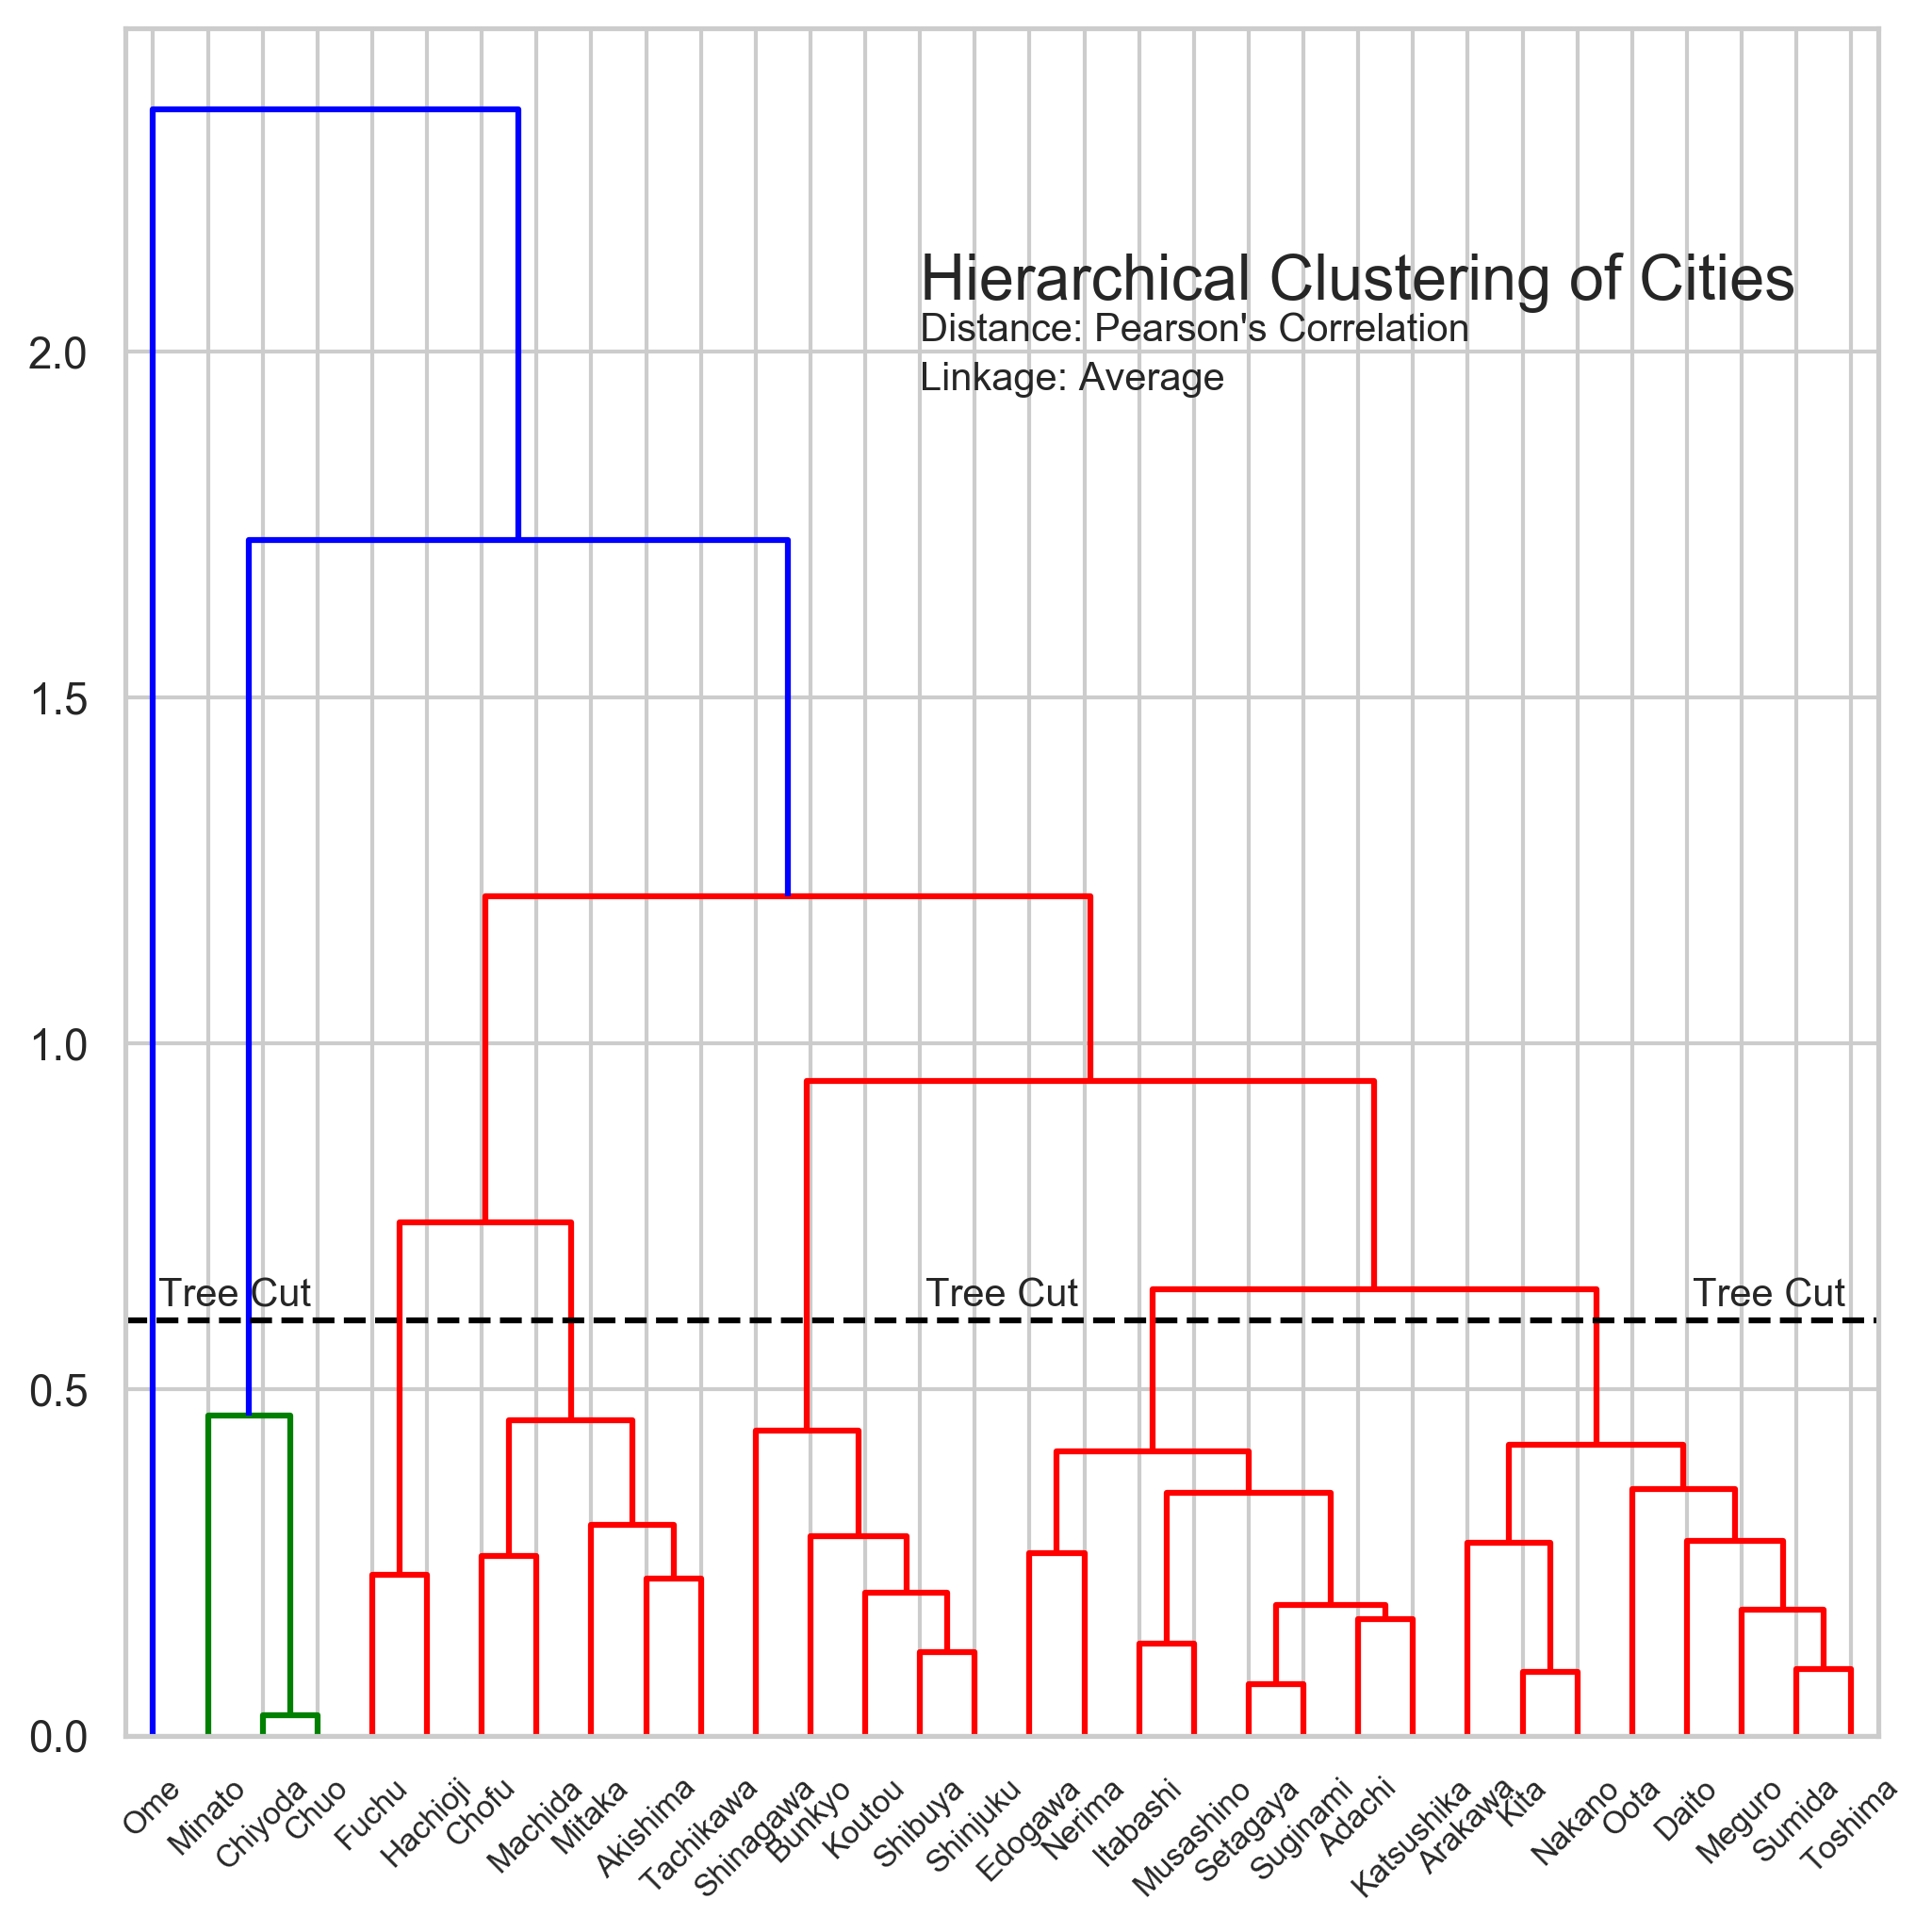
\includegraphics[height=0.85\textheight,width=0.55\textwidth]{images/Dendrogram.png}
    \end{figure}
\end{frame}

\begin{frame}{Data Analysis 2: Floating Population}
    \begin{figure}
        \centering
        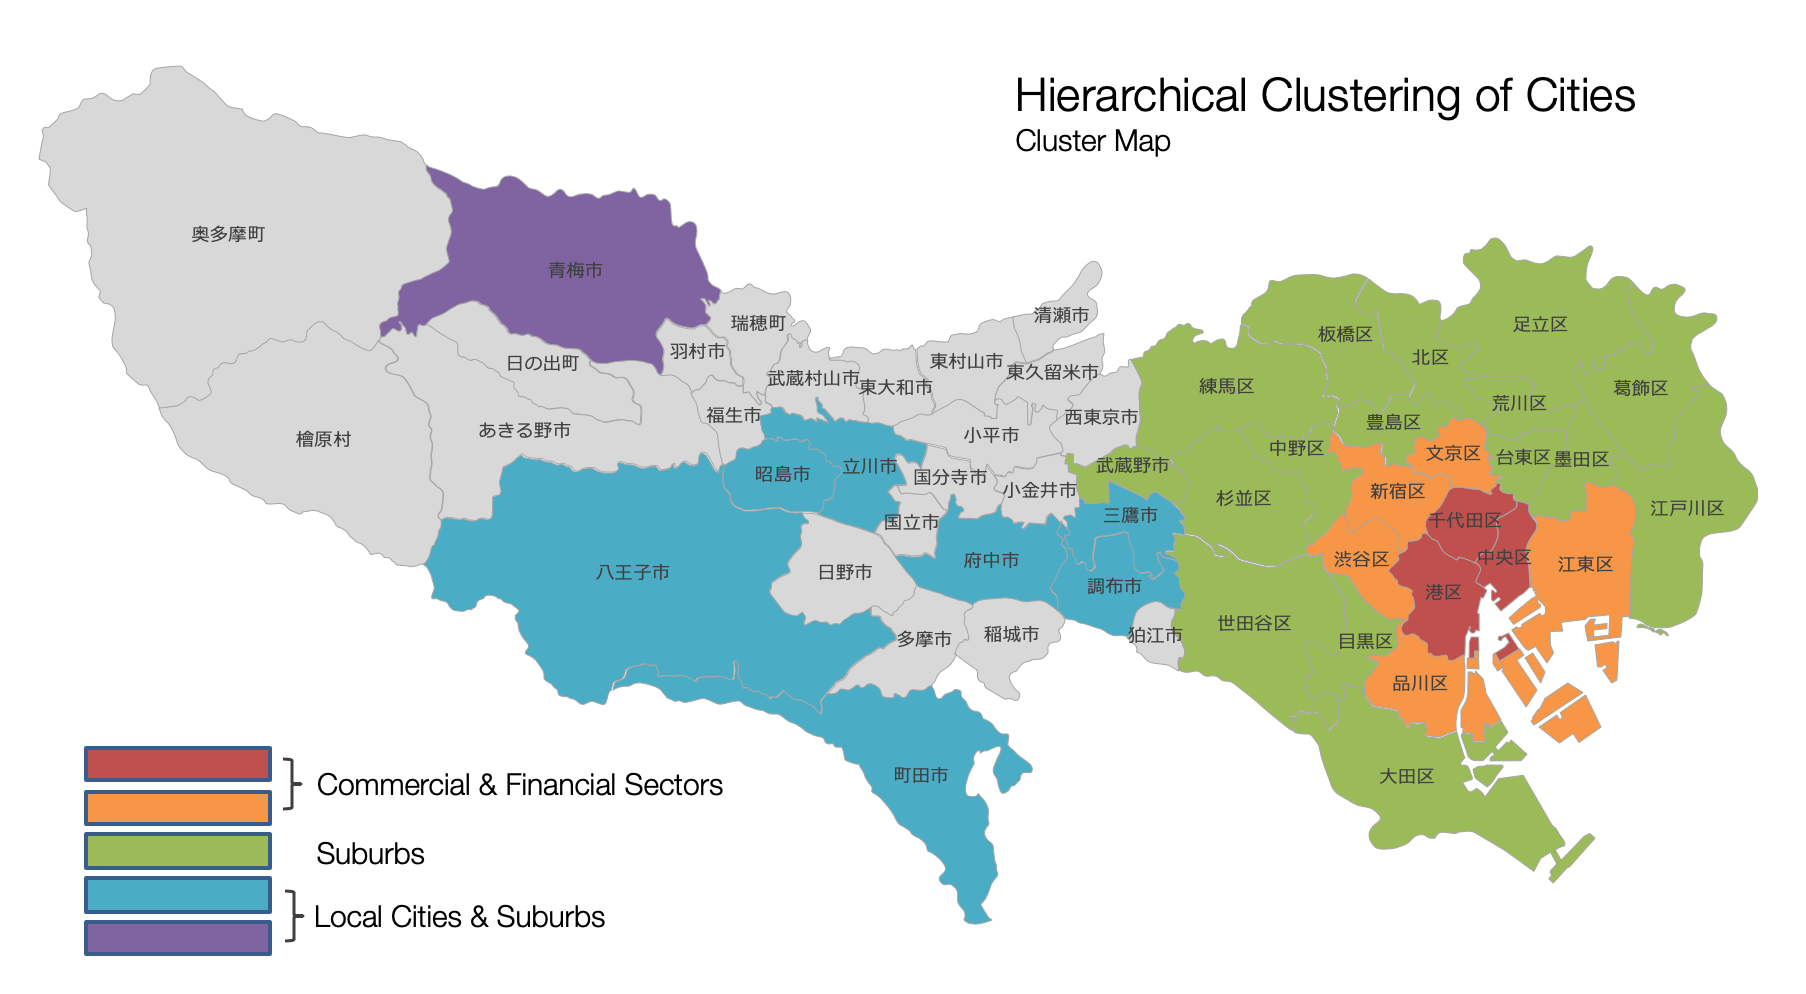
\includegraphics[height=0.85\textheight,width=0.9\textwidth]{images/cluster_map.png}
    \end{figure}
\end{frame}

\begin{frame}{Data Analysis 2: Floating Population}
    \begin{figure}
        \centering
        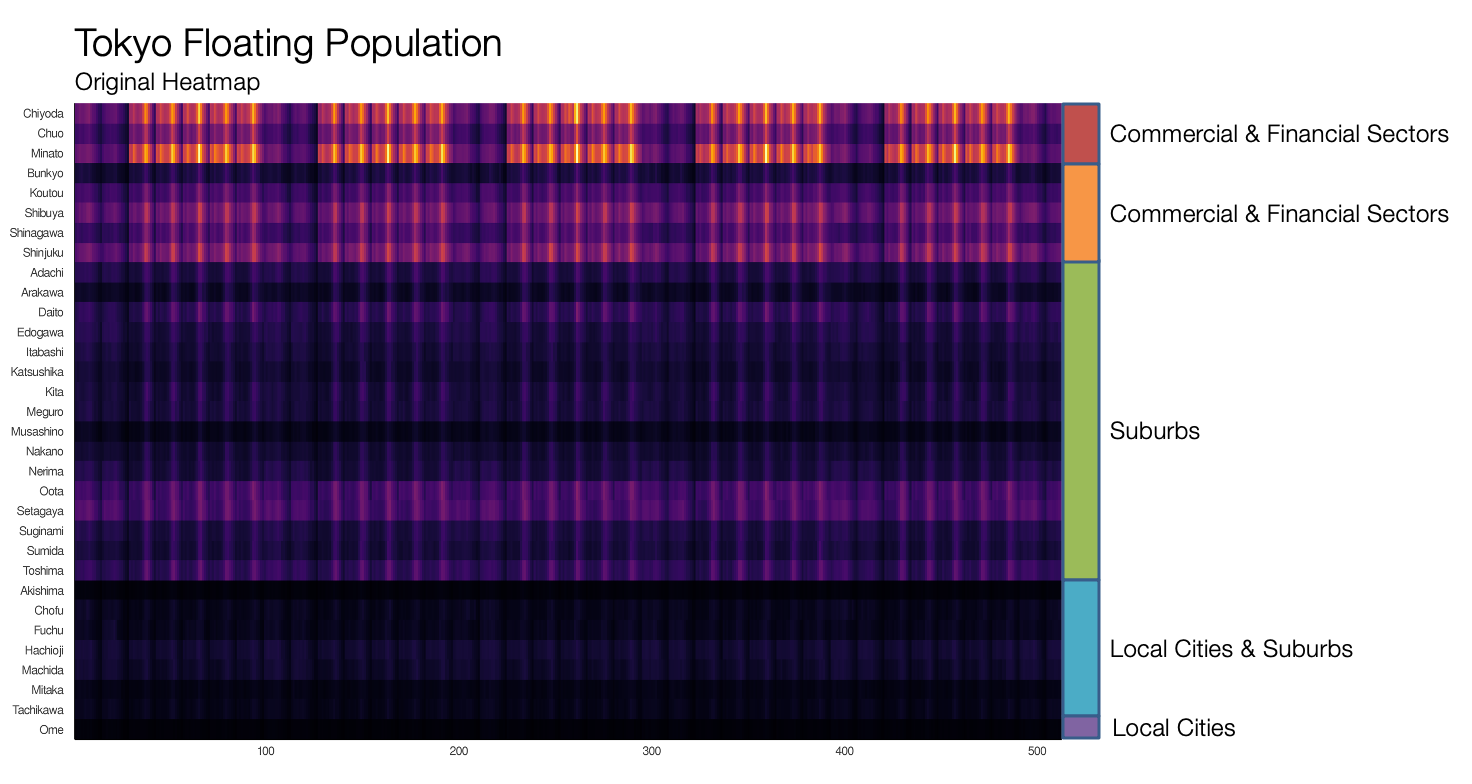
\includegraphics[height=0.8\textheight, keepaspectratio]{images/original.png}
    \end{figure}
\end{frame}

\begin{frame}{Data Analysis 2: Floating Population}
    \begin{figure}
        \centering
        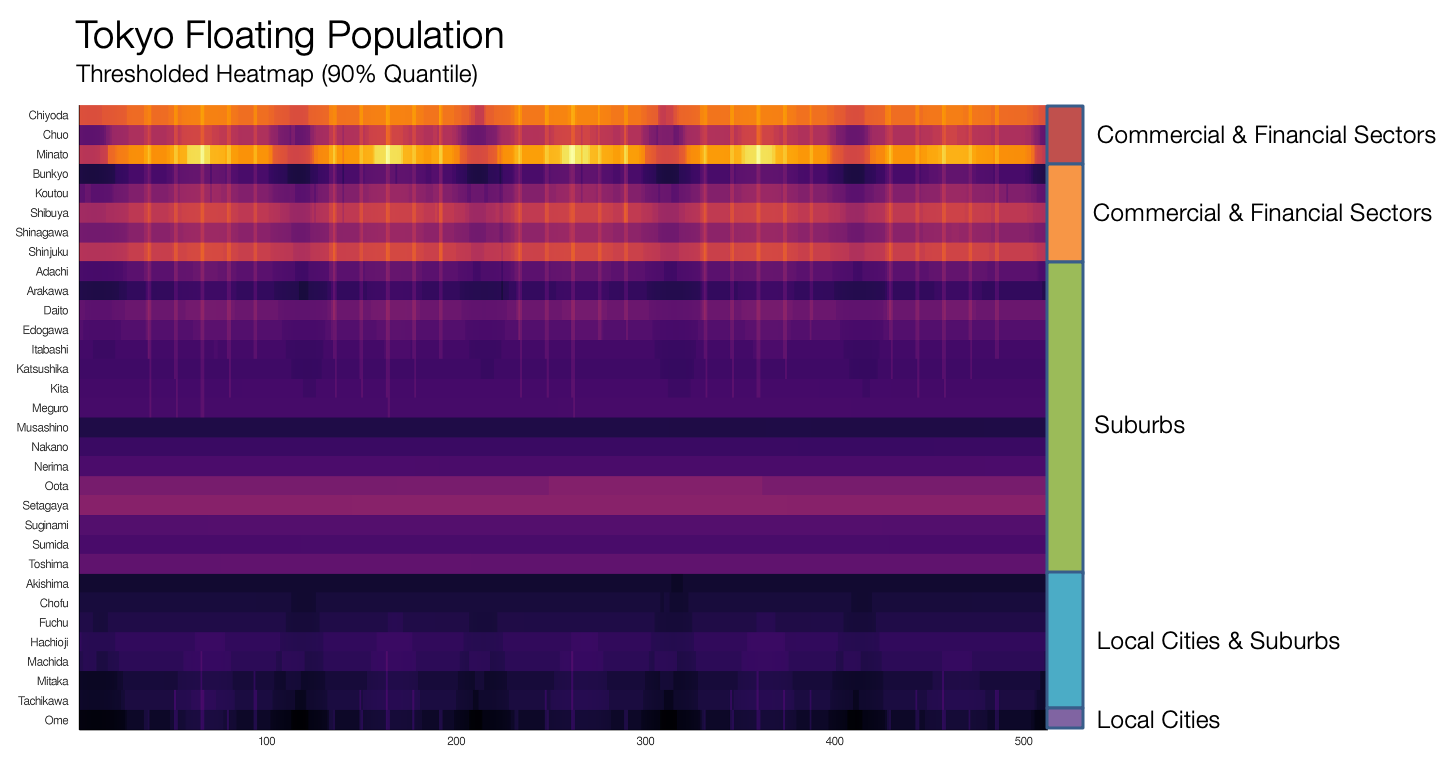
\includegraphics[height=0.8\textheight, keepaspectratio]{images/threshold90.png}
    \end{figure}
\end{frame}

\begin{frame}
\frametitle{Summary}
\begin{itemize}
    \item Wavelets are functions that contain frequency and time information
    \item We can represent signals with a basis of wavelets
    \item The advantages of the autocorrelation wavelet transform is that it is both
    shift-invariant and symmetric
    \item Some useful applications of the 2D autocorrelation wavelet transform are denoising and trend analysis
\end{itemize}
\end{frame}

\end{document}